% Use only LaTeX2e, calling the article.cls class and 12-point type.

\documentclass[12pt]{article}

% Users of the {thebibliography} environment or BibTeX should use the
% scicite.sty package, downloadable from *Science* at
% www.sciencemag.org/about/authors/prep/TeX_help/ .
% This package should properly format in-text
% reference calls and reference-list numbers.

\usepackage{scicite}
\usepackage{graphicx}
\usepackage{amsmath}
\usepackage[usenames,dvipsnames,table]{xcolor}
\usepackage[nolists,tablesfirst, nomarkers]{endfloat}

% Use times if you have the font installed; otherwise, comment out the
% following line.

\usepackage{times}

% The preamble here sets up a lot of new/revised commands and
% environments.  It's annoying, but please do *not* try to strip these
% out into a separate .sty file (which could lead to the loss of some
% information when we convert the file to other formats).  Instead, keep
% them in the preamble of your main LaTeX source file.


% The following parameters seem to provide a reasonable page setup.

\topmargin 0.0cm
\oddsidemargin 0.2cm
\textwidth 16cm 
\textheight 21cm
\footskip 1.0cm


%The next command sets up an environment for the abstract to your paper.

\newenvironment{sciabstract}{%
\begin{quote} \bf}
{\end{quote}}


% If your reference list includes text notes as well as references,
% include the following line; otherwise, comment it out.

\newcommand{\CC}[0]{\emph{cmplxcruncher}}
\newcommand{\task}[1]{\texttt{\bfseries\scshape\textcolor{MidnightBlue}{#1}}}
\newcommand{\un}[1]{\operatorname{#1}}
\newcommand{\unclassrate}[0]{\un{kpb/s/core}}
\renewcommand\refname{References and Notes}
\renewcommand{\thefootnote}{\Roman{footnote}}

% The following lines set up an environment for the last note in the
% reference list, which commonly includes acknowledgments of funding,
% help, etc.  It's intended for users of BibTeX or the {thebibliography}
% environment.  Users who are hand-coding their references at the end
% using a list environment such as {enumerate} can simply add another
% item at the end, and it will be numbered automatically.

\newcounter{lastnote}
\newenvironment{scilastnote}{%
\setcounter{lastnote}{\value{enumiv}}%
\addtocounter{lastnote}{+1}%
\begin{list}%
{\arabic{lastnote}.}
{\setlength{\leftmargin}{.22in}}
{\setlength{\labelsep}{.5em}}}
{\end{list}}


% Include your paper's title here

\title{Supplemental material of ``Microbiota: are you sick?''} 


% Place the author information here.  Please hand-code the contact
% information and notecalls; do *not* use \footnote commands.  Let the
% author contact information appear immediately below the author names
% as shown.  We would also prefer that you don't change the type-size
% settings shown here.

\author
{Jose Manuel Mart\'i,$^{1}$ Daniel M. Mart\'inez,$^{2}$ Manuel Pe\~na$^{1}$, C\'esar Gracia$^{1}$, \\
Amparo Latorre$^{2,3,4}$, Andr\'es Moya$^{2,3,4}$ \& Carlos P. Garay$^{1,\ast}$\\
\\
\normalsize{$^{1}$Instituto de Fisica Corpuscular, CSIC-UVEG, P.O.  22085, 46071, Valencia, Spain.}\\
\normalsize{$^{2}$FISABIO, Avda de Catalunya, 21, 46020, Valencia, Spain.}\\
\normalsize{$^{3}$Cavanilles Institute of Biodiversity and Evolutionary Biology, Univ. de Valencia, 46980, Spain.}\\
\normalsize{$^{4}$CIBER en Epidemiolog\' ia y Salud P\'ublica (CIBEResp), Madrid, Spain.}\\
\\
\normalsize{$^\ast$To whom correspondence should be addressed; E-mail:  penya@ific.uv.es}
}

% Include the date command, but leave its argument blank.

\date{}

%%%%%%%%%%%%%%%%% END OF PREAMBLE %%%%%%%%%%%%%%%%



\begin{document} 

% Double-space the manuscript.

\baselineskip24pt

% Make the title.

\maketitle 




% In setting up this template for *Science* papers, we've used both
% the \section* command and the \paragraph* command for topical
% divisions.  Which you use will of course depend on the type of paper
% you're writing.  Review Articles tend to have displayed headings, for
% which \section* is more appropriate; Research Articles, when they have
% formal topical divisions at all, tend to signal them with bold text
% that runs into the paragraph, for which \paragraph* is the right
% choice.  Either way, use the asterisk (*) modifier, as shown, to
% suppress numbering.

\section*{Model} \label{sec:model}

We model the microbial abundances across time along the lines of Blumm \textit{et al.}\cite{ranking}. The dynamics of taxon relative abundances is described by the Langevin equation: 
\begin{equation}
\dot{x_i} = F_i \cdot x_i^\alpha + V \cdot x_i^\beta \xi_i(t) - \phi(t) \cdot x_i,
\end{equation}
where F$_i$ captures the fitness of the taxon i, V corresponds to the noise amplitude and $\xi_i$(t) is a Gaussian random noise with zero mean  $<\xi_i(t)>$ = 0 and variance uncorrelated in time, $<\xi_i(t) \xi_i(t')>$ =  $\delta(t'-t)$, . The function $\phi(t)$ ensures the normalization at all times, $\sum x_i(t) = 1$, and corresponds to $\phi(t) = \sum F_i x_i^\alpha + \sum V x_i^\beta \xi_i(t)$ .
The temporal evolution of the probability that a taxon i has a relative abundance $x_i(t)$, P(x$_i$,t), is determined by the Fokker-Planck equation:
\begin{equation}
\frac{\partial P}{\partial t} = - \frac{\partial}{\partial x_i}  [(F_i \cdot x_i^\alpha - \phi(t) \cdot x_i ) \cdot P]+ \frac{1}{2} \frac{\partial^2}{\partial x_i^2} (V^2 \cdot x_i^{2\beta}\cdot P).
\end{equation}
The microbiota evolves towards a steady-state with a time-independent probability depending on the values of $\alpha$, $\beta$, F$_i$ and V. For $\alpha<1$ (otherwise, systems are always unstable), the steady-state probability may be localized in a region around a preferred value or broadly distributed over a wide range, depending on whether the fitness F$_i$  dominates or is overwhelmed by the noise amplitude V. The steady-state solution of the Fokker-Planck equation is given by:
\begin{eqnarray}
P_0 (x_i) &=& C_{ne}(\alpha,\beta,F_i,V)  \cdot x_i^{-2\beta}  \cdot \exp\Big[\frac{2F_i}{V^2}\frac{x_i^{1+\alpha-2\beta}}{1+\alpha-2\beta}-\frac{\phi_0}{V^2}\frac{x_i^{2-2\beta}}{1-\beta}\Big] \quad \textrm{if} \quad  2\beta \ne 1+\alpha, \notag \\
P_0 (x_i) &=& C_e(\alpha,\beta,F_i,V)  \cdot x_i^{\frac{2F_i}{V^2} -2\beta}  \cdot \exp\Big[\frac{\phi_0}{V^2}\frac{x_i^{2-2\beta}}{1-\beta}\Big] \quad \textrm{if} \quad  2\beta = 1+\alpha,
\notag
\end{eqnarray}
where $\phi_0 = (\sum_i F_i^{1/(1-\alpha)})^{1-\alpha}$ and C$_{ne}$ and C$_{e}$ are integrals that should be solved numerically for the parameters of interest. The ordered phase happens when the solution has a maximum in the physical interval ($0<x_i<1$). For larger V, the transition to a disordered phase happens when the maximum shifts to the unphysical region $x_i<0$, which sets the phase transition region V($\alpha,\beta,F_i$). The phase transition region can be calculated analytically in particular cases:
\begin{eqnarray}
F_i^2 &=& 4 \beta \phi_0 V^2\quad \textrm{if} \quad  \beta = \alpha \neq 1, \notag \\
F_i &=& \beta V^2\quad \textrm{if} \quad  2\beta = 1+\alpha,
\notag
\end{eqnarray}
where the first case, simplifies to $F= 3 V^2$ if $\beta = 0.75$ and the fitness of this taxon dominates in $\phi_0$. 
In many physical systems (Brownian motion is the classical example), the two terms of the Langevin equation are related.  The \emph{fluctuation--dissipation theorem} states a general relationship between the response to an external disturbance and the internal fluctuations of the system\cite{FD}. The theorem can be used as the basic formula to derive the fitness from the analysis of fluctuations 
of the microbiota, assuming that it is in equilibrium (the ordered phase).  

\section{Selection and Methods}

\subsection{Sample selection}
We have chosen studies about relevant pathologies containing metagenomic sequencing time data series of bacterial populations from humans in different healthy and non-healthy states. We have selected only those individuals who had three or more time points of data available in databases. Metadata of each study is provided in Supplementary Tables \ref{tab:diet} to \ref{tab:LEA}. All used 16S rRNA gene sequencing except for the study of the discordant kwashiorkor twins\cite{kwashiorkor} (see Supplementary Tables \ref{tab:DH} and \ref{tab:DK}) where shotgun metagenomic sequencing (SMS) and 16S rRNA were used. In the latter case we selected to work with SMS data to show that our method is valid regardless of the source of taxonomic information. Each one of the datasets was treated as follows:

\subsection{16rRNA sequences processing}
Reads from the selected studies were first quality filtered using the FastX toolkit\cite{FASTX}, allowing only those reads which had more than 25 of quality along the 75\% of the complete sequence. 16S rRNA reads were then clustered at 97\% nucleotide sequence identity (97\% ID) into operational taxonomic units (OTUs) using QIIME package software\cite{QIIME} (version 1.8) We followed open reference OTU picking workflow in all cases. The clustering method used was uclust, and the OTUs were matched against Silva database\cite{SILVA} (version 111, July 2012) and were assigned to taxonomy with an uclust-based consensus taxonomy assigner. The parameters used in this step were: similarity 0.97, prefilter percent id 0.6, max accepts 20, max rejects 500. 

\subsection{Metagenomic sequences processing}
Metagenomic shotgun (and 16S too) sequences were analyzed with LMAT (Livermore Metagenomics Analysis Toolkit) software package\cite{LMAT} (version 1.2.4, with Feb'15 release of data base \emph{LMAT-Grand}). LMAT was run using a Bull shared-memory node belonging to the team's HPC (high performance computing) cluster. It is equipped with 32 cores (64 threads available using Intel Hyper-threading technology) as it has 2 Haswell-based Xeons, the E5-2698v3@2.3 GHz, sharing half a tebibyte (0.5 TiB, that is, 512 gibibytes) of DRAM memory. This node is also provided with a card PCIe SSD as NVRAM, the P420m HHHL, with 1.4 TB, and 750000 reading IOPS, 4 KB, achieving 3.3 GB/s, which Micron kindly issued free of charge, as a sample for testing purposes. The computing node was supplied with a RAID-0 (striping) scratch disk area. We used the ``Grand'' database\footnote{In this context, ``Grand'' refers to a huge database that contains k-mers from all viral, prokaryote, fungal and protist genomes present in the NCBI database, plus Human reference genome (hg19), plus GenBank Human, plus the 1000 Human Genomes Project (HGP). This represent about 31.75 billion k-mers occupying 457.62 GB.}, release Feb'15, provided by the LMAT team. Previously to any calculation, the full database was loaded in the NVRAM. With this configuration the observed LMAT sustained sequence classification rate was $20\unclassrate$. Finally, it is worth mentioning that a complete set of Python scripts have been developed as back-end and front-end of the LMAT pipeline in order to manage the added complexity of time series analysis. 

\subsection{Taxa level selection}
We selected genus as taxonomic level for the subsequent steps of our work. In order to ensure that, between adjacent taxonomic levels, there were not crucial differences which could still be of relevance after standardization (see Section \ref{sec:stan}), we tested two different data sets. In the former, the antibiotics study\cite{antibiotic} with 16S data, we tested the differences between genus and family levels. The latter dataset tested was the kwashiorkor discordant twins study\cite{kwashiorkor} for both genus and species taxonomic levels. The Supplementary Figures \ref{fig:taxlev1} (overview) and \ref{fig:taxlev2} (detail) plot the comparison between studies (and so, 16S and SMS) and between adjacent taxonomic levels.

\begin{figure} 
  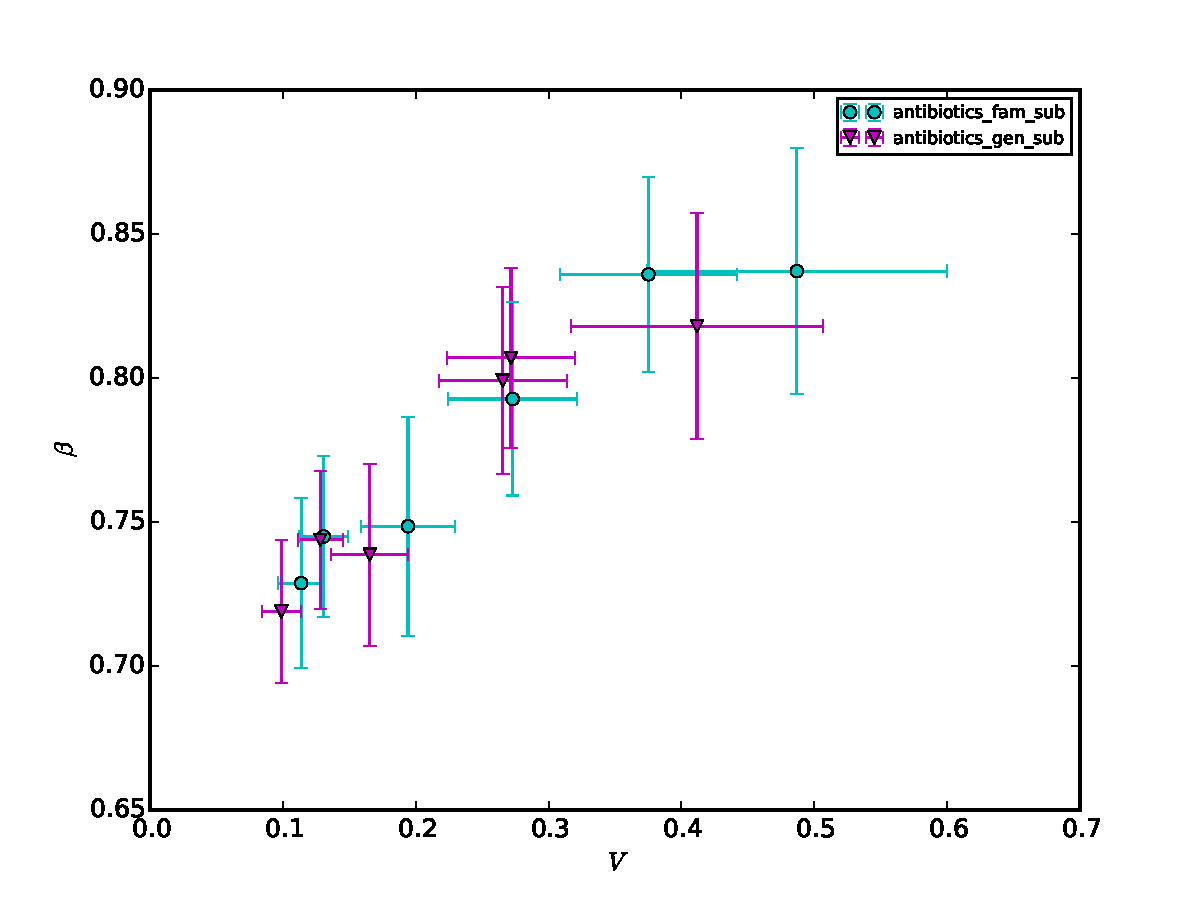
\includegraphics[width=0.5\textwidth]{results/taxalevel/sum_raw_16S.pdf}
  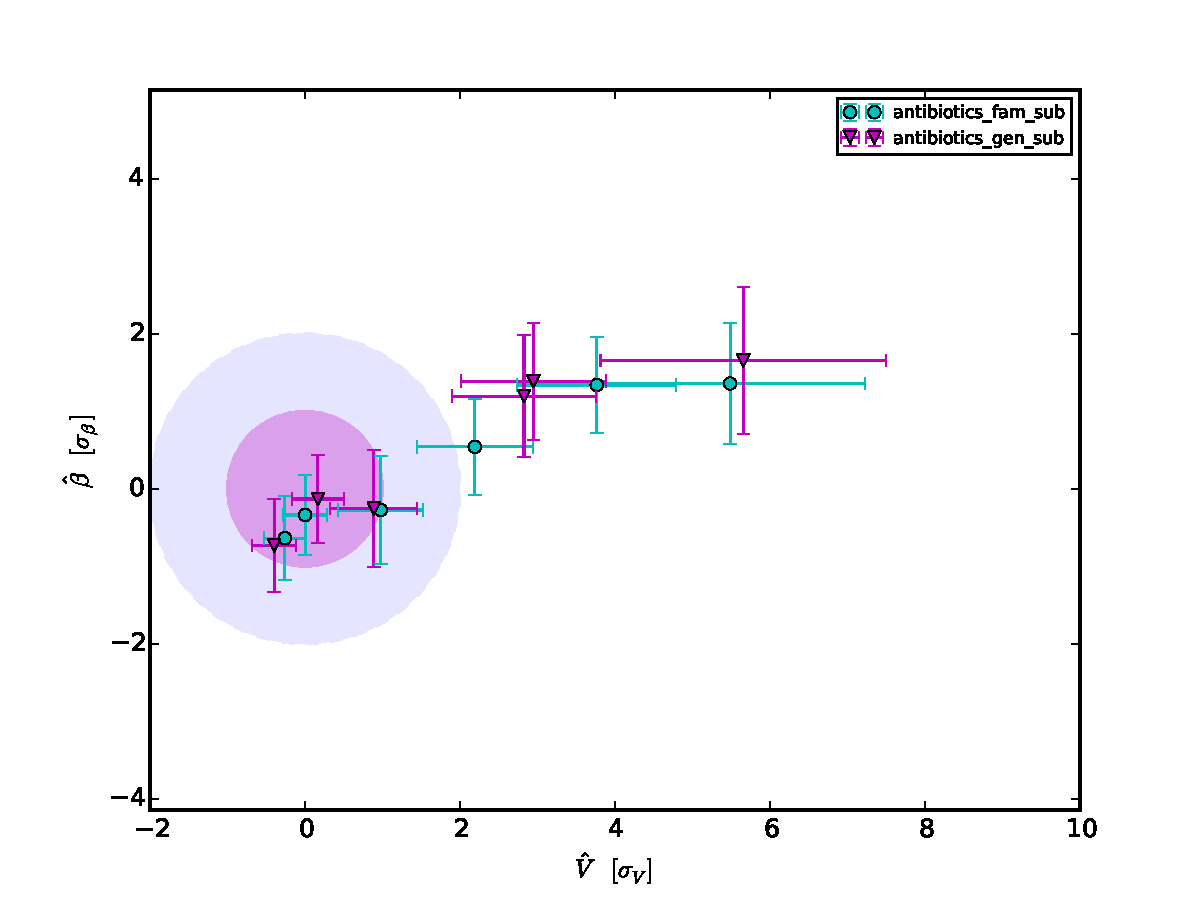
\includegraphics[width=0.5\textwidth]{results/taxalevel/sum_sta_16S.pdf}
  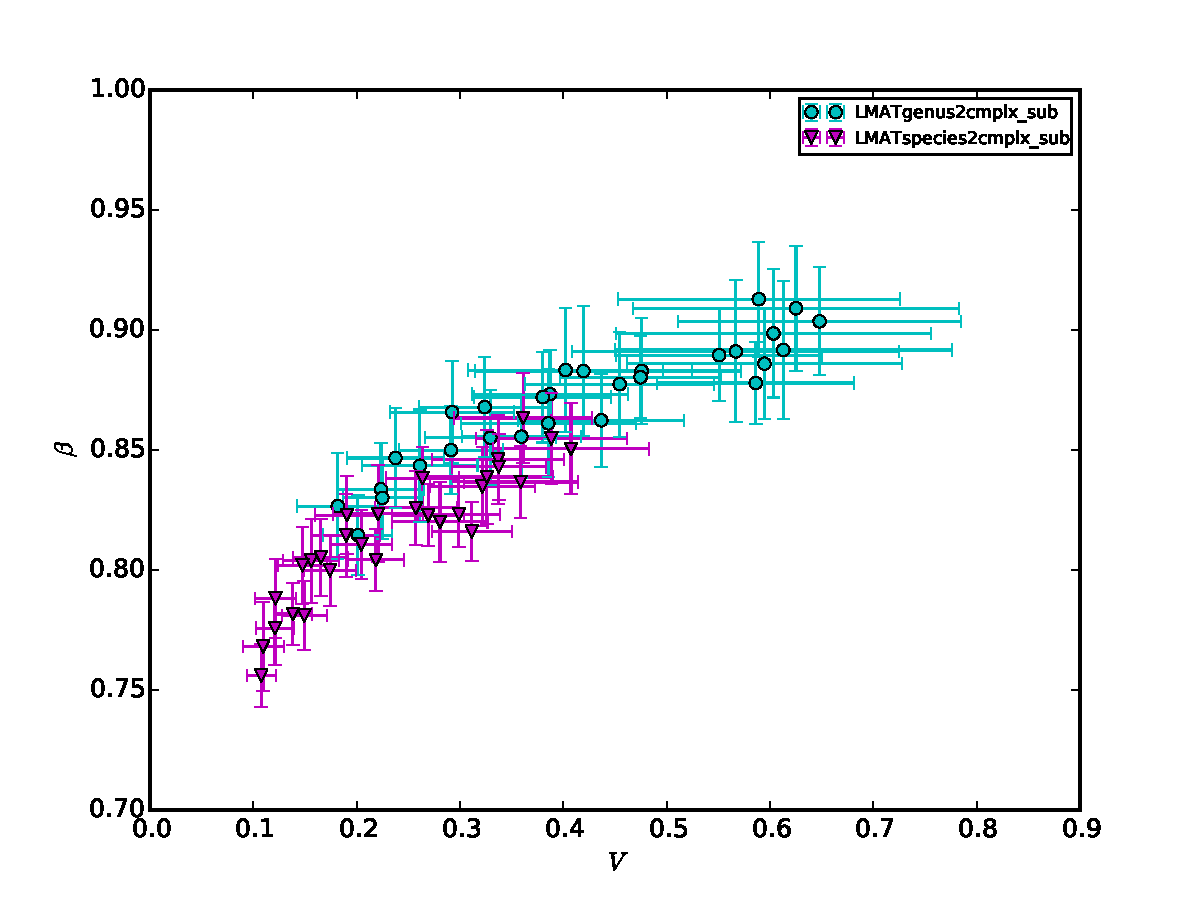
\includegraphics[width=0.5\textwidth]{results/taxalevel/sum_raw_SMS.pdf} 
  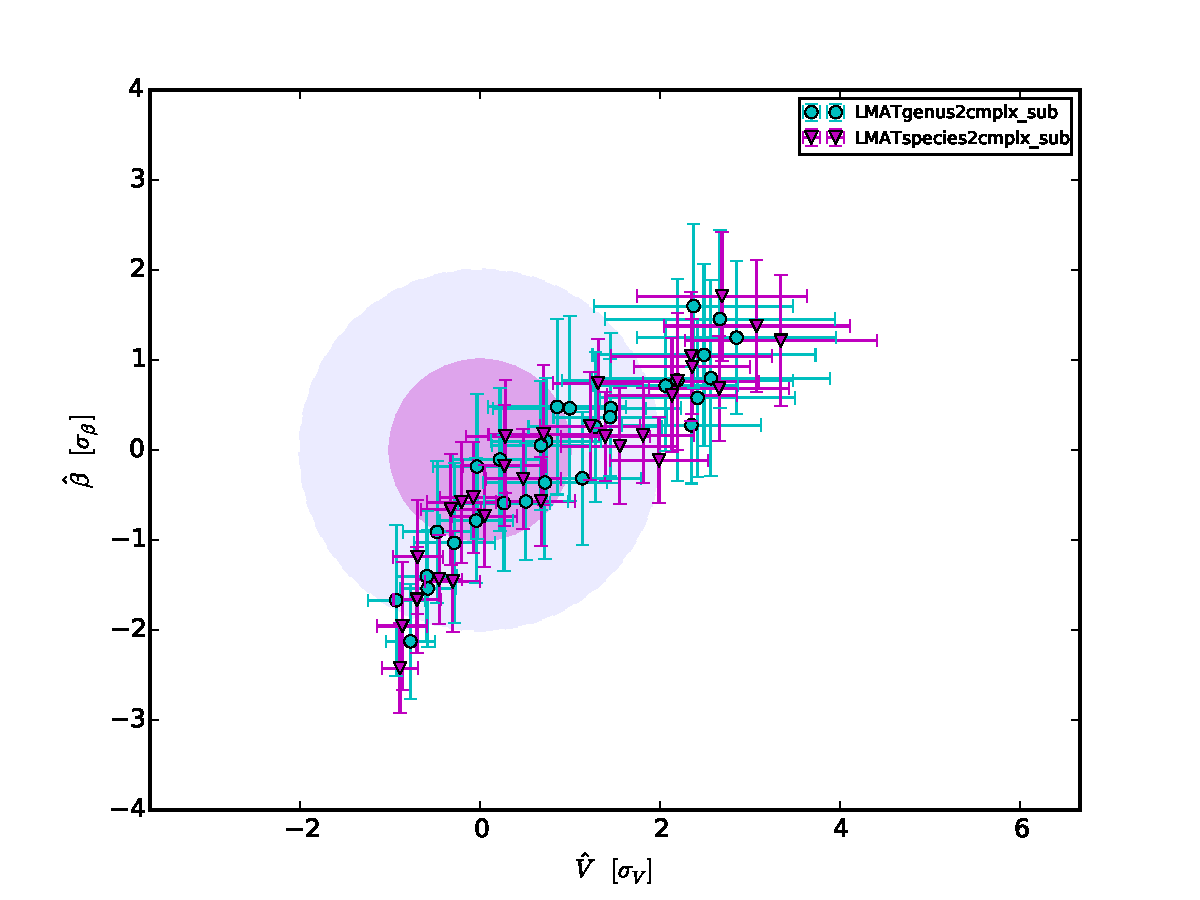
\includegraphics[width=0.5\textwidth]{results/taxalevel/sum_sta_SMS.pdf}
\caption{Overview of comparison of different approaches based on adjacent taxonomic levels using plots in the Taylor-parameters space. For 16S (former row of subfigures), the levels are family vs. genus, whereas for SMS (latter row of subfigures) levels are genus vs. species. The left column shows the raw results and the right column plots the standardized results (see Section \ref{sec:stan})}
\label{fig:taxlev1}
\end{figure}

\begin{figure} 
  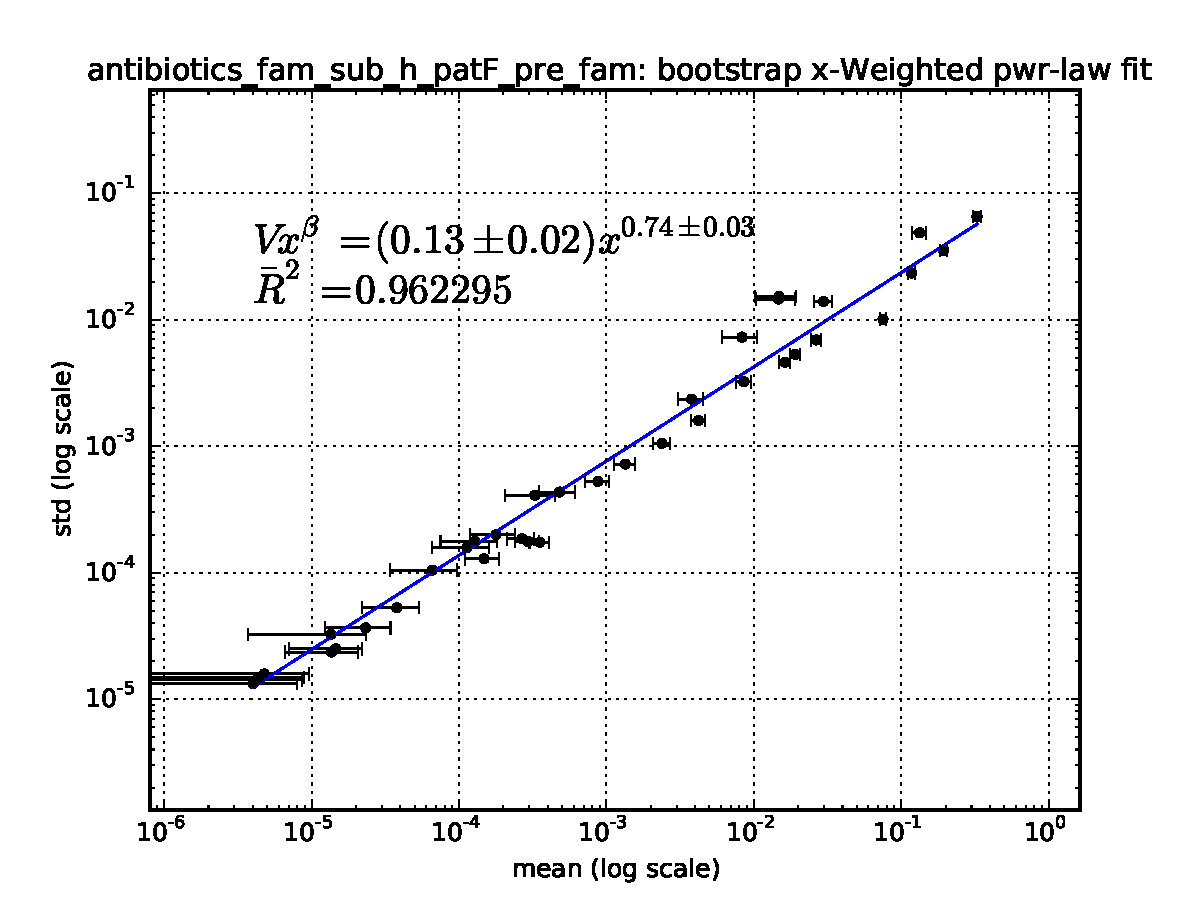
\includegraphics[width=0.5\textwidth]{results/taxalevel/xWb_fam_16S.pdf}
  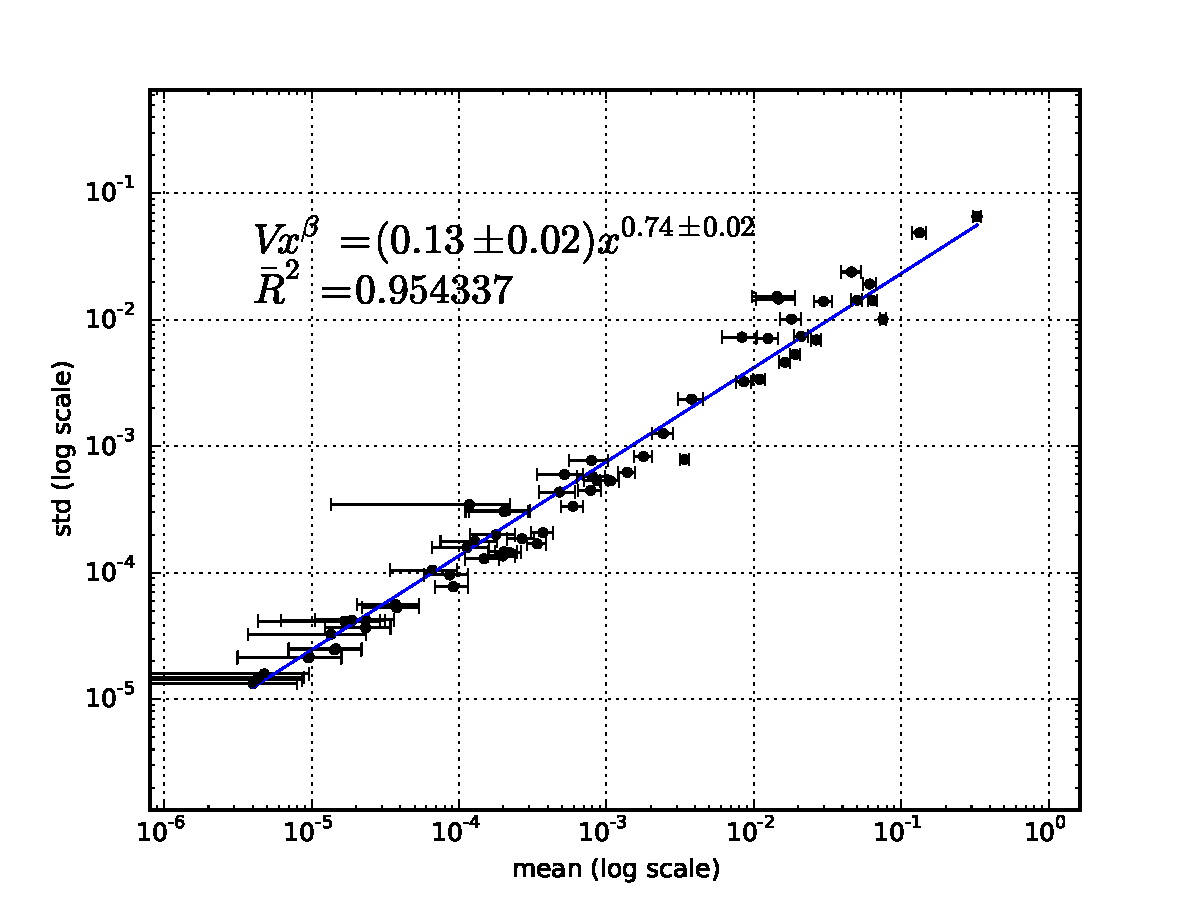
\includegraphics[width=0.5\textwidth]{results/taxalevel/xWb_gen_16S.pdf}
  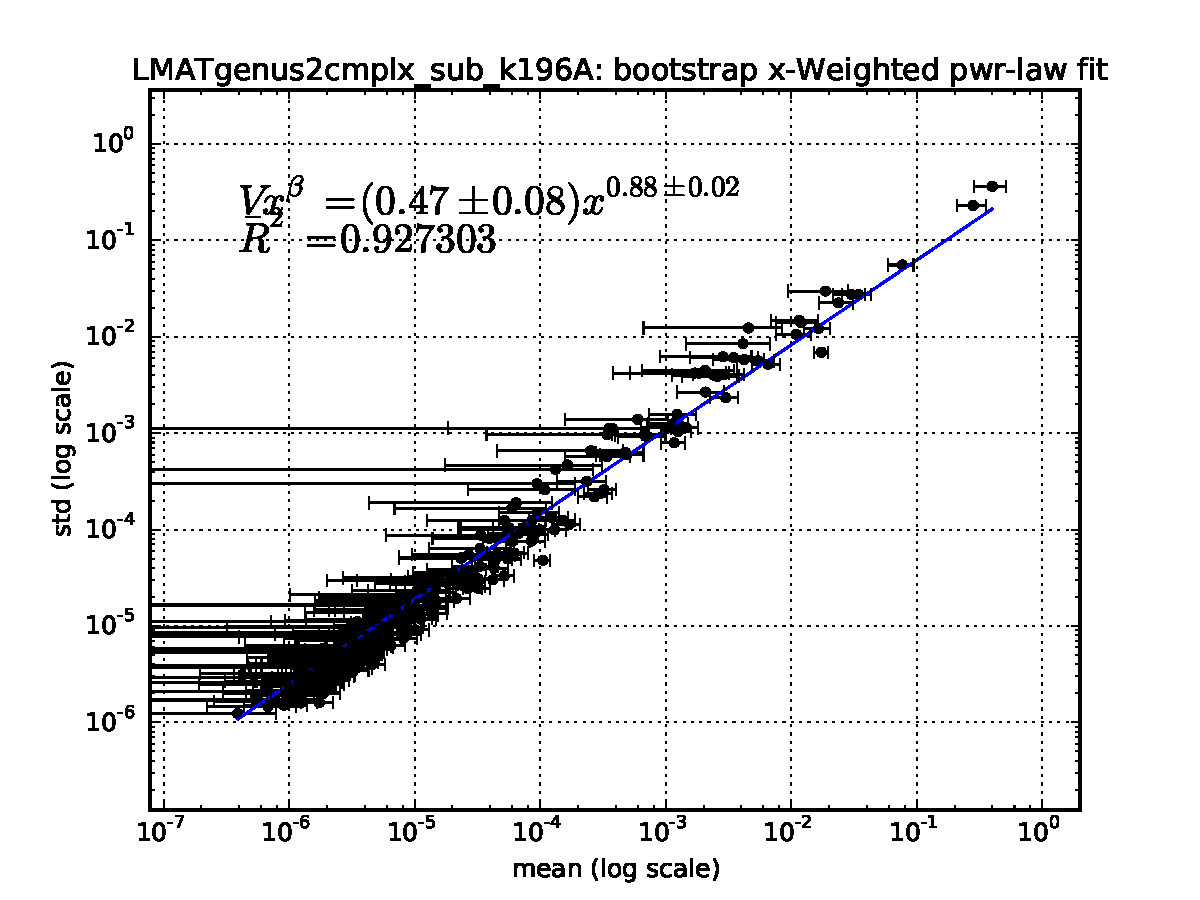
\includegraphics[width=0.5\textwidth]{results/taxalevel/xWb_gen_SMS.pdf}
  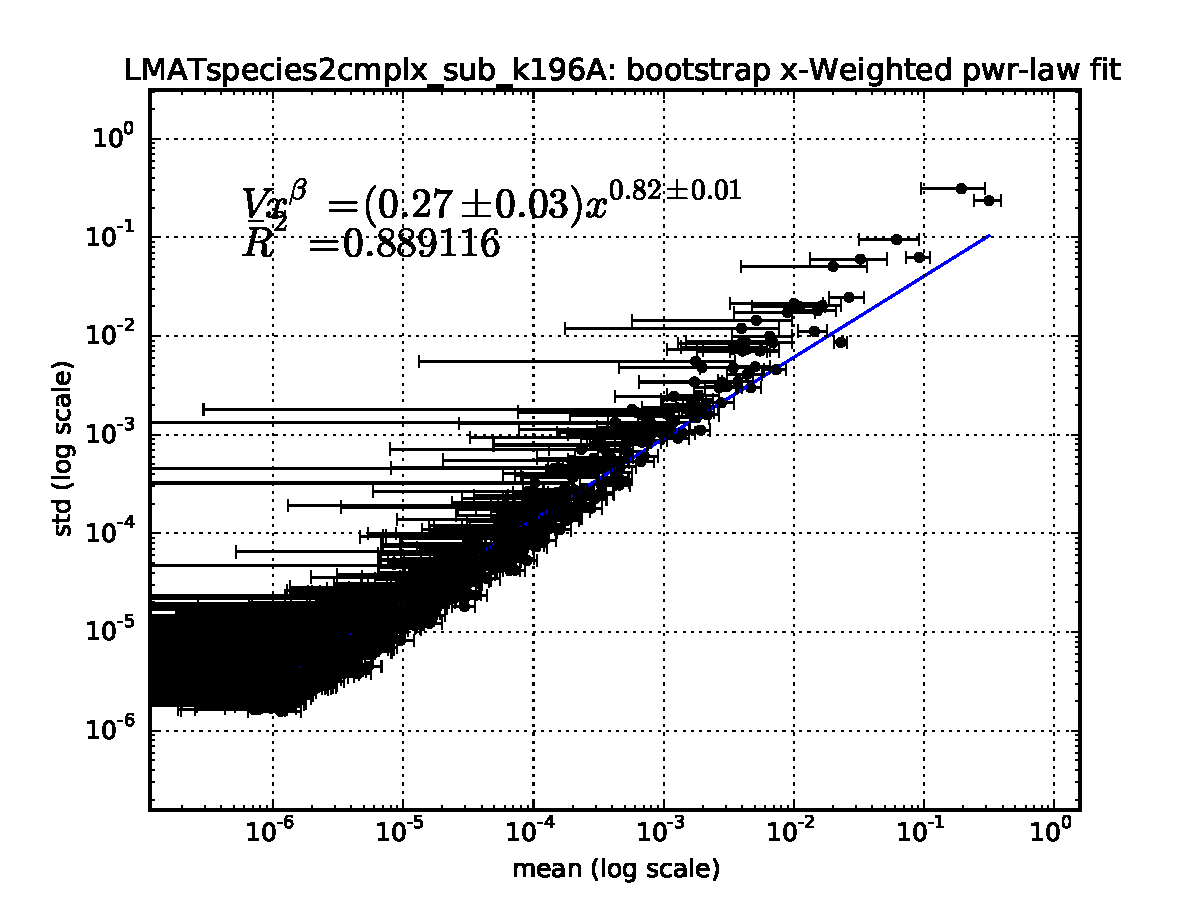
\includegraphics[width=0.5\textwidth]{results/taxalevel/xWb_spc_SMS.pdf}
\caption{Detail of comparison of different approaches based on adjacent taxonomic levels using plots of X-weighted power-law fits (see Section \ref{sec:X-w}). The former row of subfigures shows examples for 16S, whereas the latter row of subfigures plots examples for SMS. The left column shows results for the superior taxonomic level (family for 16S, genus for SMS), while the right column shows results for the inferior level (genus for 16S, specie for SMS).}
\label{fig:taxlev2}
\end{figure}

\begin{table} 
  \begin{center}
    \begin{tabular}{ccccccc}
	    \hline
		Metadata&V&$\beta$&$\bar{R}^2$&&V$_{st}$&$\beta_{st}$\\
		\hline
		A&$0.26 \pm 0.05$&$0.826 \pm 0.025$&$0.918$&&$3.1 \pm 0.9$&$1.2 \pm 0.6$\\
		A&$0.32 \pm 0.06$&$0.857 \pm 0.025$&$0.924$&&$4.4 \pm 1.1$&$2.0 \pm 0.6$\\
		A&$0.194 \pm 0.033$&$0.813 \pm 0.024$&$0.918$&&$1.9 \pm 0.6$&$0.9 \pm 0.6$\\
		A&$0.24 \pm 0.04$&$0.824 \pm 0.020$&$0.924$&&$2.7 \pm 0.7$&$1.2 \pm 0.5$\\
		A&$0.34 \pm 0.06$&$0.855 \pm 0.024$&$0.931$&&$4.7 \pm 1.1$&$1.9 \pm 0.6$\\
		A&$0.30 \pm 0.05$&$0.847 \pm 0.022$&$0.921$&&$3.9 \pm 1.0$&$1.7 \pm 0.5$\\
		A&$0.133 \pm 0.021$&$0.784 \pm 0.023$&$0.916$&&$0.7 \pm 0.4$&$0.2 \pm 0.6$\\
		A&$0.25 \pm 0.04$&$0.831 \pm 0.024$&$0.929$&&$3.0 \pm 0.8$&$1.4 \pm 0.6$\\
		\hline
		P&$0.23 \pm 0.05$&$0.804 \pm 0.035$&$0.885$&&$2.6 \pm 0.9$&$0.7 \pm 0.8$\\
		P&$0.097 \pm 0.018$&$0.705 \pm 0.031$&$0.891$&&$0.03 \pm 0.34$&$-1.6 \pm 0.7$\\
		P&$0.037 \pm 0.006$&$0.642 \pm 0.025$&$0.881$&&$-1.12 \pm 0.11$&$-3.1 \pm 0.6$\\
		P&$0.118 \pm 0.019$&$0.723 \pm 0.025$&$0.895$&&$0.4 \pm 0.4$&$-1.2 \pm 0.6$\\
		P&$0.17 \pm 0.04$&$0.78 \pm 0.04$&$0.842$&&$1.5 \pm 0.7$&$0.1 \pm 0.9$\\
		P&$0.123 \pm 0.020$&$0.757 \pm 0.026$&$0.914$&&$0.5 \pm 0.4$&$-0.4 \pm 0.6$\\
		P&$0.19 \pm 0.05$&$0.77 \pm 0.04$&$0.871$&&$1.8 \pm 0.9$&$-0.0 \pm 0.9$\\
		P&$0.121 \pm 0.020$&$0.736 \pm 0.027$&$0.921$&&$0.5 \pm 0.4$&$-0.9 \pm 0.6$\\
		P&$0.187 \pm 0.034$&$0.771 \pm 0.030$&$0.908$&&$1.8 \pm 0.7$&$-0.1 \pm 0.7$\\
		P&$0.097 \pm 0.015$&$0.735 \pm 0.025$&$0.922$&&$0.05 \pm 0.28$&$-0.9 \pm 0.6$\\
	   \hline
	   \hline
    \end{tabular}
  \end{center}
  \caption{Taylor parameters. Individuals with either animal-based (A) or plant-based (P) diets\cite{diet}. Previous to diet,  the population sampled is described by $\bar{V} = 0.09 \pm 0.05, \bar{\beta} = 0.77 \pm 0.04$.}
  \label{tab:diet}
\end{table}

 \begin{table} 
  \begin{center}
    \begin{tabular}{ccccccc}
	    \hline
		Metadata&V&$\beta$&$\bar{R}^2$&&V$_{st}$&$\beta_{st}$\\
		\hline
		Ab&$0.35 \pm 0.07$&$0.81 \pm 0.04$&$0.925$&&$4.3 \pm 1.4$&$1.3 \pm 0.9$\\
		Ab&$0.41 \pm 0.09$&$0.82 \pm 0.04$&$0.908$&&$5.6 \pm 1.8$&$1.6 \pm 0.9$\\
		Ab&$0.23 \pm 0.04$&$0.770 \pm 0.031$&$0.920$&&$2.1 \pm 0.8$&$0.5 \pm 0.7$\\
		Ab&$0.165 \pm 0.029$&$0.738 \pm 0.031$&$0.928$&&$0.9 \pm 0.6$&$-0.3 \pm 0.7$\\
		Ab&$0.34 \pm 0.06$&$0.812 \pm 0.032$&$0.936$&&$4.1 \pm 1.2$&$1.5 \pm 0.7$\\
		Ab&$0.26 \pm 0.05$&$0.798 \pm 0.033$&$0.931$&&$2.8 \pm 0.9$&$1.1 \pm 0.8$\\
	    \hline
	    \hline
    \end{tabular}
  \end{center}
  \caption{Taylor parameters for individuals taking antibiotics\cite{antibiotic}. Prior to antibiotics intake, the population sampled is described by $\bar{V} = 0.12 \pm 0.05, \bar{\beta} = 0.75 \pm 0.04$.}
  \label{tab:antibiotics}
\end{table}

\begin{table} 
  \begin{center}
    \begin{tabular}{ccccccc}
	    \hline
		Metadata&V&$\beta$&$\bar{R}^2$&&V$_{st}$&$\beta_{st}$\\
		\hline
		IBS&$0.204 \pm 0.034$&$0.739 \pm 0.029$&$0.916$&&$7.6 \pm 3.7$&$1.9 \pm 1.2$\\
		IBS&$0.35 \pm 0.05$&$0.793 \pm 0.023$&$0.935$&&$23.1 \pm 5.9$&$4.0 \pm 0.9$\\
	     \hline
	     \hline
    \end{tabular}
  \end{center}
  \caption{Taylor parameters for persons diagnosed with irritable bowel syndrome (IBS)\cite{IBS}. Healthy individuals sampled in this study are characterized by $\bar{V} = 0.134 \pm 0.009, \bar{\beta} = 0.691 \pm 0.025$.}
  \label{tab:IBS}
\end{table}

 \begin{table} 
  \begin{center}
    \begin{tabular}{ccccccc}
	    \hline
		Metadata&V&$\beta$&$\bar{R}^2$&&V$_{st}$&$\beta_{st}$\\
		\hline
		DH&$0.27 \pm 0.04$&$0.835 \pm 0.016$&$0.925$&&$0.2 \pm 0.4$&$-1.0 \pm 0.6$\\
		DH&$0.36 \pm 0.06$&$0.858 \pm 0.015$&$0.929$&&$1.1 \pm 0.6$&$-0.2 \pm 0.5$\\
		DH&$0.35 \pm 0.06$&$0.859 \pm 0.014$&$0.926$&&$1.0 \pm 0.5$&$-0.1 \pm 0.5$\\
		DH&$0.25 \pm 0.04$&$0.829 \pm 0.014$&$0.911$&&$0.0 \pm 0.4$&$-1.2 \pm 0.5$\\
		DH&$0.30 \pm 0.05$&$0.844 \pm 0.014$&$0.920$&&$0.5 \pm 0.4$&$-0.7 \pm 0.5$\\
		DH&$0.29 \pm 0.05$&$0.850 \pm 0.016$&$0.915$&&$0.4 \pm 0.5$&$-0.5 \pm 0.5$\\
		DH&$0.28 \pm 0.05$&$0.848 \pm 0.016$&$0.921$&&$0.3 \pm 0.5$&$-0.5 \pm 0.6$\\
		DH&$0.35 \pm 0.07$&$0.861 \pm 0.017$&$0.918$&&$0.9 \pm 0.6$&$-0.0 \pm 0.6$\\
		DH&$0.31 \pm 0.04$&$0.833 \pm 0.012$&$0.916$&&$0.6 \pm 0.4$&$-1.1 \pm 0.4$\\
		DH&$0.33 \pm 0.05$&$0.843 \pm 0.013$&$0.925$&&$0.8 \pm 0.5$&$-0.7 \pm 0.5$\\
		DH&$0.31 \pm 0.05$&$0.852 \pm 0.014$&$0.925$&&$0.6 \pm 0.5$&$-0.4 \pm 0.5$\\
		DH&$0.31 \pm 0.05$&$0.853 \pm 0.015$&$0.930$&&$0.6 \pm 0.5$&$-0.4 \pm 0.5$\\
		DH&$0.203 \pm 0.033$&$0.815 \pm 0.015$&$0.907$&&$-0.44 \pm 0.32$&$-1.7 \pm 0.5$\\
		\hline
    \end{tabular}
  \end{center}
  \caption{Taylor parameters for the healthy subject of the discordant twins\cite{kwashiorkor}. This table continues in Supplementary Table \ref{tab:DK}. The population of healthy twins is characterized by $\bar{V} = 0.25 \pm 0.10, \bar{\beta} = 0.863 \pm 0.028$.}
  \label{tab:DH}
\end{table}

\begin{table} 
  \begin{center}
    \begin{tabular}{ccccccc}
	    \hline
		Metadata&V&$\beta$&$\bar{R}^2$&&V$_{st}$&$\beta_{st}$\\
		\hline
		DK&$0.40 \pm 0.07$&$0.859 \pm 0.017$&$0.926$&&$1.5 \pm 0.7$&$-0.1 \pm 0.6$\\
		DK&$0.44 \pm 0.08$&$0.868 \pm 0.016$&$0.919$&&$1.8 \pm 0.8$&$0.2 \pm 0.6$\\
		DK&$0.196 \pm 0.031$&$0.819 \pm 0.014$&$0.916$&&$-0.50 \pm 0.30$&$-1.5 \pm 0.5$\\
		DK&$0.160 \pm 0.026$&$0.798 \pm 0.015$&$0.904$&&$-0.85 \pm 0.25$&$-2.3 \pm 0.5$\\
		DK&$0.30 \pm 0.05$&$0.845 \pm 0.014$&$0.924$&&$0.5 \pm 0.4$&$-0.6 \pm 0.5$\\
		DK&$0.23 \pm 0.04$&$0.834 \pm 0.014$&$0.908$&&$-0.1 \pm 0.4$&$-1.0 \pm 0.5$\\
		DK&$0.27 \pm 0.05$&$0.848 \pm 0.015$&$0.930$&&$0.2 \pm 0.4$&$-0.5 \pm 0.5$\\
		DK&$0.35 \pm 0.07$&$0.860 \pm 0.019$&$0.916$&&$1.0 \pm 0.7$&$-0.1 \pm 0.7$\\
		DK&$0.34 \pm 0.05$&$0.835 \pm 0.012$&$0.917$&&$0.9 \pm 0.5$&$-1.0 \pm 0.4$\\
		DK&$0.25 \pm 0.04$&$0.831 \pm 0.012$&$0.912$&&$0.0 \pm 0.4$&$-1.1 \pm 0.4$\\
		DK&$0.36 \pm 0.06$&$0.858 \pm 0.013$&$0.918$&&$1.1 \pm 0.5$&$-0.2 \pm 0.5$\\
		DK&$0.31 \pm 0.06$&$0.851 \pm 0.016$&$0.924$&&$0.6 \pm 0.6$&$-0.4 \pm 0.6$\\
		DK&$0.149 \pm 0.022$&$0.799 \pm 0.013$&$0.905$&&$-0.96 \pm 0.22$&$-2.2 \pm 0.5$\\
	    \hline
	    \hline
    \end{tabular}
  \end{center}
  \caption{Taylor parameters for the kwashiorkor part of the discordant twins\cite{kwashiorkor}. This is a continuation of Supplementary Table \ref{tab:DH}. The population of healthy twins is characterized by $\bar{V} = 0.25 \pm 0.10, \bar{\beta} = 0.863 \pm 0.028$.}
  \label{tab:DK}
\end{table}

\begin{table} 
  \begin{center}
    \begin{tabular}{ccccccc}
	    \hline
		Metadata&V&$\beta$&$\bar{R}^2$&&V$_{st}$&$\beta_{st}$\\
		\hline
		OW&$0.59 \pm 0.12$&$0.894 \pm 0.034$&$0.920$&&$6.6 \pm 2.0$&$2.6 \pm 1.0$\\
		OW&$0.22 \pm 0.04$&$0.830 \pm 0.030$&$0.904$&&$0.5 \pm 0.6$&$0.7 \pm 0.9$\\
		\hline
		OBI&$0.28 \pm 0.04$&$0.855 \pm 0.022$&$0.958$&&$1.5 \pm 0.6$&$1.4 \pm 0.6$\\
		OBI&$0.33 \pm 0.07$&$0.870 \pm 0.031$&$0.916$&&$2.4 \pm 1.1$&$1.9 \pm 0.9$\\
		\hline
		OBII&$0.223 \pm 0.032$&$0.823 \pm 0.023$&$0.938$&&$0.6 \pm 0.5$&$0.5 \pm 0.7$\\
		OBII&$0.208 \pm 0.029$&$0.844 \pm 0.022$&$0.935$&&$0.4 \pm 0.5$&$1.1 \pm 0.7$\\
		\hline
		OBIII&$0.34 \pm 0.05$&$0.855 \pm 0.025$&$0.943$&&$2.5 \pm 0.9$&$1.4 \pm 0.7$\\
		OBIII&$0.26 \pm 0.04$&$0.845 \pm 0.026$&$0.954$&&$1.1 \pm 0.7$&$1.2 \pm 0.8$\\
		OBIII&$0.33 \pm 0.06$&$0.870 \pm 0.027$&$0.908$&&$2.4 \pm 1.0$&$1.9 \pm 0.8$\\
		OBIII&$0.200 \pm 0.026$&$0.843 \pm 0.020$&$0.949$&&$0.2 \pm 0.4$&$1.1 \pm 0.6$\\
		OBIII&$0.30 \pm 0.05$&$0.846 \pm 0.026$&$0.929$&&$1.9 \pm 0.8$&$1.2 \pm 0.7$\\
		OBIII&$0.176 \pm 0.029$&$0.826 \pm 0.026$&$0.894$&&$-0.2 \pm 0.5$&$0.6 \pm 0.8$\\
		OBIII&$0.30 \pm 0.06$&$0.841 \pm 0.031$&$0.896$&&$1.8 \pm 0.9$&$1.0 \pm 0.9$\\
		OBIII&$0.28 \pm 0.04$&$0.857 \pm 0.025$&$0.941$&&$1.5 \pm 0.7$&$1.5 \pm 0.7$\\
		OBIII&$0.122 \pm 0.018$&$0.822 \pm 0.024$&$0.930$&&$-1.05 \pm 0.30$&$0.5 \pm 0.7$\\
		\hline
		OBIIId&$0.47 \pm 0.08$&$0.872 \pm 0.023$&$0.945$&&$4.7 \pm 1.3$&$1.9 \pm 0.7$\\
		OBIIId&$0.38 \pm 0.06$&$0.846 \pm 0.023$&$0.951$&&$3.2 \pm 1.0$&$1.2 \pm 0.7$\\
		OBIIId&$0.36 \pm 0.06$&$0.842 \pm 0.022$&$0.954$&&$2.9 \pm 0.9$&$1.1 \pm 0.6$\\
	    \hline
	    \hline
    \end{tabular}
  \end{center}
  \caption{Taylor parameters for individuals with different degrees of overweight and obesity\cite{LEA}. Healthy people in this study, whom were not obese, are characterized by $\bar{V} = 0.19 \pm 0.06, \bar{\beta} = 0.806 \pm 0.034$.}
  \label{tab:LEA}
\end{table}


\section{Temporal evolution of model parameters}

We have studied the time dependence of the variability $V$ and power law index $\beta$ (see Section \ref{sec:model}) by using a sliding window approach. The total number of time points are divided in subsets of five points, where next subset is defined by adding next time sampling and by eliminating the earliest one. Both parameters were calculated for each subset against the average time lapse. Figure \ref{fig:tempevo1} shows the variability  $V$ as a function of time for the largest sampling: two individuals in the Caporaso's study\cite{moving} corresponding to the gut microbiota of a male (upper plot) and a female (lower plot). Figure \ref{fig:tempevo2} shows the time evolution of $V$ for patient P2 of the IBS study\cite{IBS} (upper plot) and patient D in the antibiotics study\cite{antibiotic} (lower plot). 

\begin{figure}
	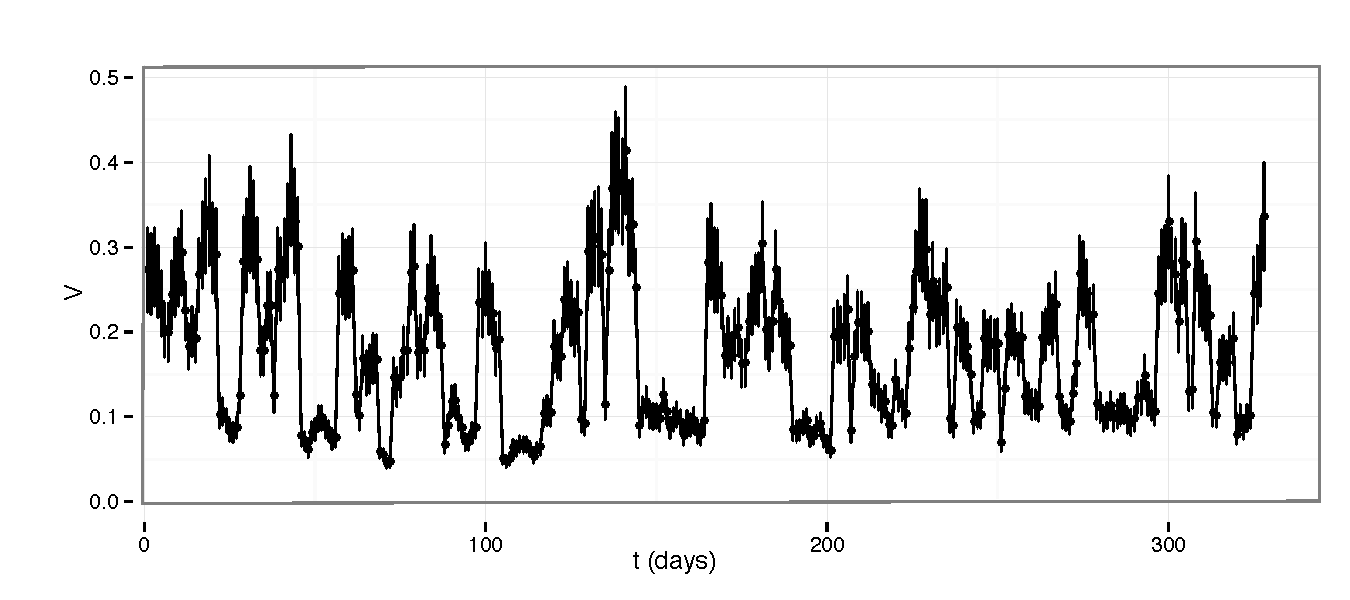
\includegraphics[width=1.0\textwidth]{results/sliwin/male_mov.pdf}
	\hspace*{3mm}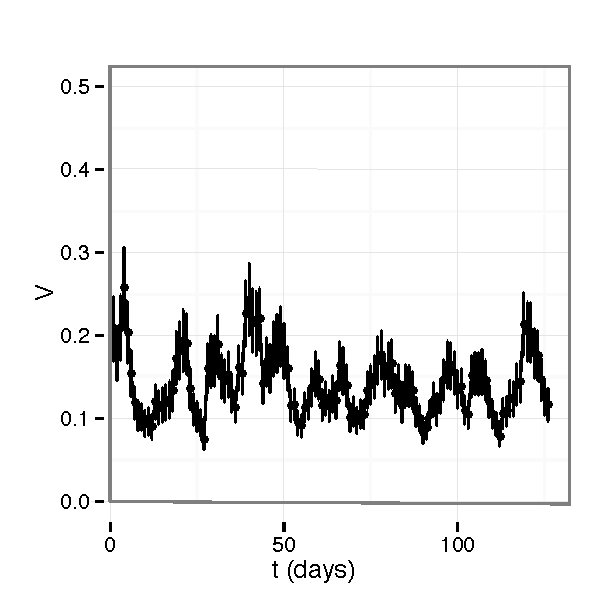
\includegraphics[width=0.448\textwidth]{results/sliwin/female_mov.pdf}
\caption{$V$ as a function of time for the two individuals in the Caporaso's study\cite{moving}: samples of gut microbiome of a male (upper plot) and a female (lower plot). Both samples show changes in the variability V with quasi--periodic behavior peaked at about 10 days. Variability grows more for the gut microbiota of the male and share a minimal value around 0.1 with the gut microbiota of the female.}
\label{fig:tempevo1}
\end{figure}

\begin{figure}
	\centering 
 	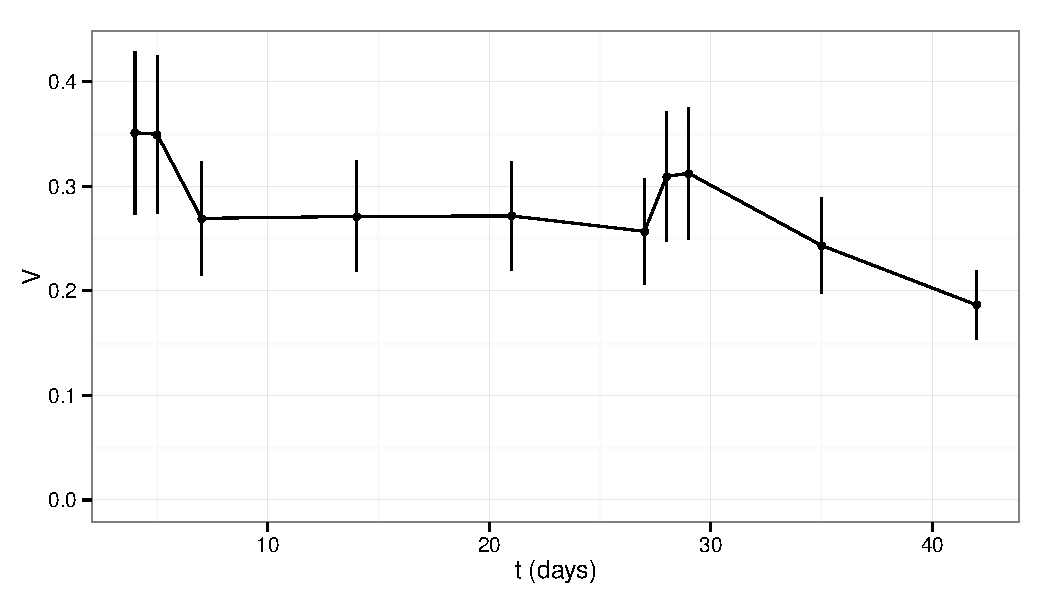
\includegraphics[width=0.8\textwidth]{results/sliwin/patP2_IBS.pdf}
  	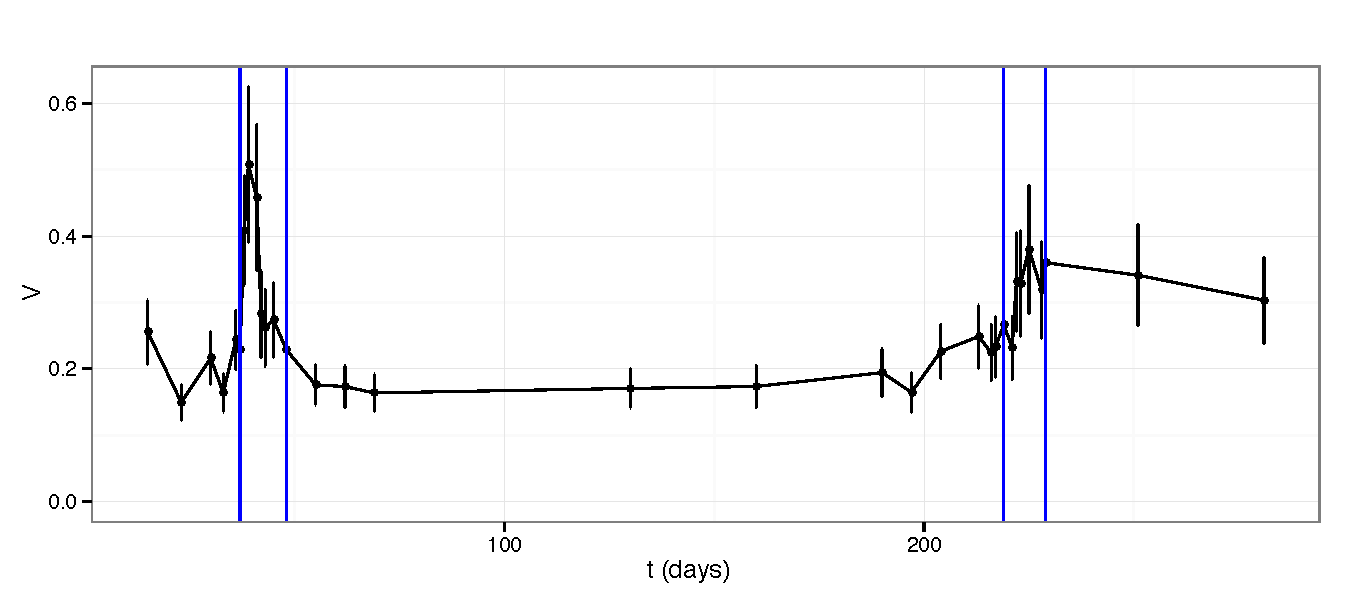
\includegraphics[width=1.0\textwidth]{results/sliwin/patD_antibio.pdf} 
\caption{$V$ as a function of time for patient P2 of the IBS study\cite{IBS} (upper plot) and patient D in the antibiotics study\cite{antibiotic} (lower plot). The variability 
of the gut microbiota of P2 decreases from above 0.3 to below 0.2, showing a slow tendency to increase the order of the system.  Antibiotic intake leaks to a quick increase of variability which lasts for a few days to recover ordering. The second antibiotic treatment shows some memory (lower increase of variability) with a slower recovery. NOTE: The blue vertical lines in the lower plot are showing the periods of antibiotic treatment.}
\label{fig:tempevo2}
\end{figure}

\section{Engineered Software}

A complete software framework, named 'ComplexCruncher', has been engineered to support the analysis of the dynamics of ranking processes in complex systems. Although the software was devised with a clear bias towards metagenomics, it is general enough to be able to cope with a ranking process in any complex system. Implemented in Python using well-known open-source community software, the software solution is composed of two parts that can be used together or apart: a web-based graphic front-end connected to a database, and a computing kernel. Used together, this software enables other users to reproduce our results easily and, furthermore, upload and analyse their own data or experiment with the preloaded metagenomics data sets. The next sections of this supplementary material deal with these two software pieces in detail.

\section{Web-based front-end}

`ComplexCruncher WebPortal' (CCWebPortal) is a web platform designed to allow the user to interact with a data repository of selected and well-documented metagenomics data sources. Through a few simple steps, the user can perform advanced searches on the complete set of records in the metagenomics repository.  The web application provides advanced filters that allow the user to reduce the search to a small set of interest. After this first step, the user can refine the search and discard those records that do not meet certain requirements.

The web application allows calculations to be done directly by the stable release of the \CC\ computing kernel. At the end of the calculations, the results are displayed to the user on the same browser which runs the web application. Then, the user can interact over the series of generated graphics thus allowing flexible comparison among them. In addition, CCWebPortal enables direct download of generated data (plots, spreadsheets, etc). The web application generates a report file summarizing all the results in PDF format. If the user has login permissions, CCWebPortal enables the option of insert new database records in addition to editing and deleting existing ones.

CCWebPortal is a web application that runs on current versions of many browsers. Additional software is not needed and only requires javaScript to be enabled on the browser to run applications. CCWebPortal is, at least, compatible with the following browsers: Internet Explorer 6+, Firefox 3.6+ (PC, Mac), Safari 4+, Chrome 10+ and Opera 11+ (PC, Mac).

CCWebPortal is implemented following the client$-$server distributed programming model. The user connects to the website and a set of javaScript files are downloaded and executed on the local machine. Subsequently, the client application connects to a remote server that enables the execution of calculations and transactions through a centralized database management system. The web application is deployed on the client side using ExtJs libraries. ExtJs is a javaScript development framework to implement interactive Web applications using AJAX, DHTML and DOM technologies. ExtJS has been widely adopted by large technology projects worldwide. Its success lies in its ability to design and implement web interfaces with a clear and flexible functionality for the end user. ExtJs is used under the GNU license GPL v3.

The CCWebPortal website communicates with a remote server that hosts a MySQL database. The database runs on a MyISAM engine that optimizes the speed of access to records in a transactional web-based environment. A set of relational tables allows the structuring of the metagenomics repository to establish relationships between records. Thus the search and information threshing is optimized for queries launched from the client interface. Access to the database on the server is implemented through Django framework. Django is an open-source framework written in Python using the model-view-controller (MVC) architectural pattern for implementing user interfaces, which eases the development and updating of code. This framework is used to implement web applications on the server side and allows flexible and modular developments and access to various types of database managers. Django runs as a web server, awaiting requests from the client CCWebPortal application. Once a user is authorized to perform a given operation, Django interacts with the database serving queries to the client application.

\section{Computing kernel}

The effective data analysis has been performed with a Python tool developed from scratch following the OOP\footnote{Object Oriented Programming, but OOP also stands for Object Oriented Python, which is applicable here too.} paradigm, called \CC. This software is the back-end of the website described in the previous subsection. However, it could be run as an independent piece of software since it is built as a Python package provided with a command-line front-end (\CC.py). Once installed, the tool can be run interactively (using the flag \texttt{-i}/\texttt{--interactive}) but also in automatic mode (flag \texttt{-a}/\texttt{--automatic} followed by the desired graphic format, e.g., \texttt{pdf}, \texttt{png}, \texttt{svg}, \texttt{ps}), which uses parallel computation to speed up the analysis of several data sources. 

The external mandatory dependencies of \CC\ are with Python packages \emph{pandas}, \emph{matplotlib}, \emph{numpy}, \emph{scipy} and \emph{xlrd}, while the recommended ones are \emph{pylatex} and \emph{uncertainties}. The PEP8 compliant code of \CC\ could be executed under a Python 2.7 interpret, but a 3.X interpret is strongly advised. The complete distribution of \CC\ has the code signature shown in the Table \ref{tab:cloc}, obtained through the \emph{CLOC}\footnote{\emph{Count Lines of Code} is a perl script that counts blank lines, comment lines, and physical lines of source code.} tool release 1.62. Figure \ref{fig:CC} shows the code layout of the complete distribution of \CC.

\begin{table}
  \begin{center}
    \begin{tabular}{lrrrrcrcr}
    \hline
	Language & files & blank & comment & code & x & scale & = & 3rd gen. equiv \\
	\hline
	Python & 13 & 384 & 666 & 4222 &x& 4.20 &=& 17732.40 \\
	R & 1 & 11 & 38 & 192 &x& 3.00 &=& 576.00 \\	
	\hline
	SUM: & 14 & 395 & 704 & 4414 &x& 4.15 &=& 18308.40 \\
	\hline
    \end{tabular}
  \end{center}
  \caption{Line counting for the complete distribution of \CC\ by \emph{CLOC}}
  \label{tab:cloc}
\end{table}

\begin{figure}
  \centering
	\[ \text{\task{ComplexCruncher}}
	\begin{cases}
		\text{\task{cmplxcruncher.py}} \\
		\\ 
		\text{\task{cmplxcruncher}}
		\begin{cases}
			\text{\task{\_\_init\_\_.py}} \\ 
			\\ 
			\text{\task{models.py}} \\
			\\ 
			\text{\task{plots.py}} \\
			\\ 
			\text{\task{sessions.py}} \\ 
		\end{cases}
		\\ \\
		\text{\task{tools}}
		\begin{cases}
			\text{\task{power\_analysis.R}} \\
			\\ 
			\text{\task{rawlmat2lmat.py}} \\
			\\ 
			\text{\task{lmat2cmplx.py}} \\
			\\ 
			\text{\task{pyLMAT\_rl.py}} \\
			\\ 
			\text{\task{pyLMAT\_cs.py}} \\
			\\ 
			\text{\task{pyLMAT\_gl.py}} \\
			\\
			\text{\task{LMAT}}
			\begin{cases}
	    		\text{\task{pyLMAT\_rescore.py}} \\ 
	    		\\ 
	    		\text{\task{HMPspiker.py}} 
			\end{cases}
		\end{cases}
	\end{cases} \]
	\caption{\CC\ layout}
	\label{fig:CC}
\end{figure}


\CC\ performs the power-law fit described in the \emph{Blumm, N. et al.} paper, but by fitting the best model, i.e. choosing between fitting a power-law using linear regression versus nonlinear regression\cite{ecology}. In the power-law fit plots we also show the generalized coefficient of determination computed for continuous models\cite{genR2,disR2}.

\section{Un-weighted power-law fit}\label{sec:unw}

\subsection{Fitting the best model}

As mentioned above, to choose between fitting power laws ($y=Vx^\beta$) using linear regression on log-transformed (LLR) data versus non-linear regression (NLR), we mainly follow \emph{General Guidelines for the Analysis of Biological Power Laws}\cite{ecology}. It consists of the following three steps:
\begin{enumerate}
    \item Determining the appropriate error structure by likelihood analysis.
    \begin{enumerate}
        \item Fit the Non-Linear Regression (NLR) model and obtain $V_\text{NLR}$, $\beta_\text{NLR}$ and $\sigma_\text{NLR}^2$.
        \item Calculate the loglikelihood that the data ($n$ is sample size) are generated from a normal distribution with additive error:
        \begin{itemize}
            \item The likelihood of a normal distribution is:  
            $$\mathcal{L}_\text{norm} = \prod_{i=1}^n\left[\frac{1}{\sqrt{2\pi\sigma^2_\text{NLR}}}\;\exp{\left(-\frac{\left(y_i-V_\text{NLR}x_i^{\beta_\text{NLR}}\right)^2}{2\sigma^2_\text{NLR}}\right)}\right]$$
            \item So, the loglikelihood of a normal distribution is:
            \begin{eqnarray*}
                \log\mathcal{L}_\text{norm} &=& -\frac{n}{2}\log\left|2\pi\sigma^2_\text{NLR}\right| - \frac{1}{2\sigma^2_\text{NLR}}\underbrace{\sum_{i=1}^n\left(y_i-V_\text{NLR}x_i^{\beta_\text{NLR}}\right)^2}_{\mathrm{RSS
                }_\text{NLR}}\\
                &=& -\frac{n}{2}\log\left|2\pi\sigma^2_\text{NLR}\right|-\frac{\mathrm{RSS}_\text{NLR}}{2\sigma^2_\text{NLR}}
            \end{eqnarray*}
        \end{itemize}
        \item Calculate the \emph{corrected Akaike's Information Criterion} for the NLR model:
        $$\mathrm{AIC_{c_{NLR}}} = 2k - 2\log\mathcal{L}_\text{norm} + \frac{2k(k+1)}{n-k-1}$$
        \item Fit the Log-transformed Linear Regression (LLR) model and obtain $V_\text{LLR}$, $\beta_\text{LLR}$ and $\sigma_\text{LLR}^2$.
        \item Calculate the loglikelihood that the data ($n$ is sample size) are generated from a lognormal distribution with multiplicative error:
        \begin{itemize}
            \item The likelihood of a lognormal distribution is: 
            $$\mathcal{L}_\text{logn} = \prod_{i=1}^n\left[\frac{1}{y_i\sqrt{2\pi\sigma^2_\text{LLR}}}\;\exp{\left(-\frac{\left(\log|y_i|-\log|V_\text{LLR}|-\beta_\text{LLR}\log|x_i|\right)^2}{2\sigma^2_\text{LLR}}\right)}\right]$$
            \item So, the loglikelihood of a lognormal distribution is: 
            \begin{eqnarray*}
                \log\mathcal{L}_\text{logn} &=& -\frac{n}{2}\log\left|2\pi\sigma^2_\text{LLR}\right| - \sum_{i=1}^n\log|y_i| -\\
                &&\qquad-\frac{1}{2\sigma^2_\text{LLR}}\underbrace{\sum_{i=1}^n\left(\log|y_i|-\log|V_\text{LLR}|-\beta_\text{LLR}\log|x_i|\right)^2}_{\mathrm{RSS
                }_\text{LLR}}\\
                &=& -\frac{n}{2}\log\left|2\pi\sigma^2_\text{LLR}\right| - \frac{\mathrm{RSS}_\text{LLR}}{2\sigma^2_\text{LLR}} - \sum_{i=1}^n\log|y_i|
            \end{eqnarray*}
        \end{itemize}
        \item Calculate the \emph{corrected Akaike's Information Criterion} for the LR model: 
        	$$\mathrm{AIC_{c_{LLR}}} = 2k - 2\log\mathcal{L}_\text{logn} + \frac{2k(k+1)}{n-k-1}$$
    \end{enumerate}
    \item Compare $\mathrm{AIC_{c_{NLR}}}$ with $\mathrm{AIC_{c_{LLR}}}$:
    \begin{itemize}
        \item If $\mathrm{AIC_{c_{NLR}}} - \mathrm{AIC_{c_{LLR}}} < -2$, the assumption of normal error is favoured compared to lognormal error, so proceed with the results obtained from the NLR fit.
        \item If $\mathrm{AIC_{c_{NLR}}} - \mathrm{AIC_{c_{LLR}}} > 2$, the assumption of lognormal error is favoured compared to normal error, so proceed with the results obtained from the LLR fit.
        \item If $\left|\mathrm{AIC_{c_{NLR}}} - \mathrm{AIC_{c_{LLR}}}\right| \leq 2$, no model is favoured, so proceed with averaging:
        \begin{eqnarray*}
            B_\text{av} &=& w_\text{NLR}V_\text{NLR} + w_\text{LLR}V_\text{LLR} \\
            \beta_\text{av} &=& w_\text{NLR}\beta_\text{NLR} + w_\text{LLR}\beta_\text{LLR}
        \end{eqnarray*}
        where: 
        \begin{eqnarray*}
            w_\text{NLR} &=& \frac{1}{1+\mathrm{e}^{\frac{1}{2}\left(\mathrm{AIC_{c_{NLR}}}-\mathrm{AIC_{c_{LLR}}}\right)}} \\
            w_\text{LLR} &=& \frac{1}{1+\mathrm{e}^{\frac{1}{2}\left(\mathrm{AIC_{c_{LLR}}}-\mathrm{AIC_{c_{NLR}}}\right)}}
        \end{eqnarray*}
        which are obtained to fulfill the next condition: $w_\text{NLR} + w_\text{LLR} = 1$. The CIs for $B_\text{av}$ and $\beta_\text{av}$ are to be generated by ordinary bootstrapping\footnote{\CC\ has available the next bootstrapping alternatives\cite{boot}: ordinary, ``Resampling Residuals'' method, ``Wild'' method, and ``Monte-Carlo'' method.}.      
    \end{itemize}
    \item Assess the validity of the underlying statistical assumptions with diagnostic plots because while it is rare for all the assumptions to be fully satisfied by real-life data sets, major violations indicate the lack of appropriateness of the model and, thus, the potential invalidity of the results.
\end{enumerate}

\subsection{Calculating the coefficient of determination}

We think the best approach in this situation is to apply the generalized $R^2$ that, for continuous models, was defined as\cite{genR2}:
$$ R^2 = 1 - \left(\frac{\mathcal{L}(0)}{\mathcal{L}(\hat\theta)}\right)^{\!\!\frac{2}{n}} $$
where $\mathcal{L}(\hat\theta)$ and $\mathcal{L}(0)$  denote the likelihoods of the fitted and the ``null'' model, respectively, and $n$ is the sample size. In terms of the loglikelihoods, the generalized coefficient of determination would be:
$$ R^2 = 1 - \mathrm{e}^{-\frac{2}{n}\left(\log\mathcal{L}(\hat\theta)-\log\mathcal{L}(0)\right)} $$
We have the likelihoods calculated from the previous section, but what about the ``null'' models? We understand that they are the models with only the intercept. So for the Gaussian additive error model:
$$\mathcal{L}_\text{norm}(0) = \prod_{i=1}^n\left[\frac{1}{\sqrt{2\pi\sigma^2_\text{NLR0}}}\;\exp{\left(-\frac{\left(y_i-\bar y\right)^2}{2\sigma^2_\text{NLR0}}\right)}\right]$$
So:
\begin{eqnarray*}
\log\mathcal{L}_\text{norm}(0) &=& -\frac{n}{2}\log\left|2\pi\sigma^2_\text{NLR0}\right| - \frac{1}{2\sigma^2_\text{NLR0}}\sum_{i=1}^n\left(y_i-\bar y\right)^2\\
 &=& -\frac{n}{2}\left(\log\left|2\pi\sigma^2_\text{NLR0}\right| + 1 \right)
\end{eqnarray*}
since $\sigma^2_\text{NLR0}=\frac{1}{n}\sum\left(y_i-\bar y\right)^2=\frac{1}{n}\mathrm{TSS}_\text{NLR}$. Now, coming back to the coefficient of determination, we have:
\begin{eqnarray*}
R^2_\text{NLR} &=& 1 - \mathrm{e}^{\frac{2}{n}\left(\log\mathcal{L}_\text{NLR}(0)-\log\mathcal{L}_\text{NLR}(\hat\theta)\right)} = 1 - \exp{\left(\frac{\log(\mathrm{RSS}_\text{NLR})}{\log(\mathrm{TSS}_\text{NLR})}\right)}
 =\\ &=& 1 - \frac{\mathrm{RSS}_\text{NLR}}{\mathrm{TSS}_\text{NLR}} =
 1 - \frac{\sum_{i=1}^n\left(y_i-V_\text{NLR}x_i^{\beta_\text{NLR}}\right)^2}{\sum_{i=1}^n\left(y_i-\bar y\right)^2}
\end{eqnarray*}
recovering the traditional expression for $R^2$. Using the same approach for calculating $R^2_\text{LLR}$, then:
$$\mathcal{L}_\text{logn}(0) = \prod_{i=1}^n\left[\frac{1}{y_i\sqrt{2\pi\sigma^2_\text{LLR0}}}\;\exp{\left(-\frac{\left(\log|y_i|-\log|B_\text{LLR0}|\right)^2}{2\sigma^2_\text{LLR0}}\right)}\right]$$
So:
\begin{eqnarray*}
\log\mathcal{L}_\text{logn}(0) &=& -\frac{n}{2}\log\left|2\pi\sigma^2_\text{LLR0}\right| - \frac{1}{2\sigma^2_\text{LLR0}}\sum_{i=1}^n\left(\log|y_i|-\overline{\log|y|}\right)^2 - \sum_{i=1}^n\log|y_i|\\
 &=& -\frac{n}{2}\left(\log\left|2\pi\sigma^2_\text{LLR0}\right| + 1 \right) - \sum_{i=1}^n\log|y_i|
\end{eqnarray*}
since $\sigma^2_\text{LLR0}=\frac{1}{n}\sum\left(\log|y_i|-\overline{\log|y|}\right)^2=\frac{1}{n}\mathrm{TSS}_\text{logn}$. Again, recalling the expression for the generalized coefficient of determination, we have:
\begin{eqnarray*}
R^2_\text{LLR} &=& 1 - \mathrm{e}^{\frac{2}{n}\left(\log\mathcal{L}_\text{LLR}(0)-\log\mathcal{L}_\text{LLR}(\hat\theta)\right)} = 1 - \exp{\left(\frac{\log(\mathrm{RSS}_\text{LLR})}{\log(\mathrm{TSS}_\text{LLR})}\right)}
 =\\ &=& 1 - \frac{\mathrm{RSS}_\text{LLR}}{\mathrm{TSS}_\text{LLR}} =
 1 - \frac{\sum_{i=1}^n\left(\log|y_i|-\log|V_\text{LLR}|-\beta_\text{LLR}\log|x_i|\right)^2}{\sum_{i=1}^n\left(\log|y_i|-\overline{\log|y|}\right)^2}
\end{eqnarray*}


\section{X-weighted power-law fit}\label{sec:X-w}

When fitting the power-law of std vs. mean, we can take into account that every mean has uncertainty and estimate it for a sample size $n$ by the SEM (\emph{Standard Error of the Mean}):
$$ \mathrm{SEM} = \frac{s}{\sqrt{n}}$$
where $s$ is the sample standard deviation. So, the vector of weights is computed with:
$$ \mathbf{w} = \frac{1}{\overrightarrow{\mathrm{SEM}}} = \frac{\sqrt{\mathbf{n}}}{\mathbf{s}}$$

Here, the uncertainties affect the independent variable, so the fit is not so trivial as a Y-weighted fit, where the uncertainties affect the dependent variable. A standard approach to do this fit is: a) invert your variables before applying the weights, b) then perform the weighted fit, and finally, c) revert the inversion. This method is deterministic, but the approximate solution worsens with smaller $R^2$. For comparison, we develop a stochastic method by using a bootstrapping-like strategy that avoids the inversion and is applicable regardless of $R^2$. Both methods, detailed below, are implemented in \CC.

\subsection{Method 1: By inverting the data}

In the case of the log-LR model, we have:
$$\log y = \log V + \beta\log x \quad\rightarrow\quad \underbrace{\log x}_{\tilde y} = \overbrace{-\frac{1}{\beta}\log V}^{b} + \overbrace{\frac{1}{\beta}}^{m}\underbrace{\log y}_{\tilde x}$$ 
where $m$ determines the slope or gradient of the fitted line, and $b$ determines the point at which the line crosses the y-axis, otherwise known as the y-intercept. Once the model is fitted, the original parameters can be retrieved easily:
\begin{eqnarray*}
\beta &=& \frac{1}{m} \\
V &=& \mathrm{e}^{-\beta b} = \mathrm{e}^{-\frac{b}{m}}
\end{eqnarray*}
Their respective uncertainties are to be obtained using \emph{error propagation}:
\begin{eqnarray*}
    \sigma_\beta &=& \left|\frac{\mathrm{d}\beta}{\mathrm{d}m}\right|\sigma_m \quad=\quad \frac{1}{m^2}\;\sigma_m \\
    \sigma_V &=& \sqrt{\left(\frac{\partial V}{\partial b}\right)^{\!\!2}\sigma_b^2 +
      \left(\frac{\partial V}{\partial m}\right)^{\!\!2}\sigma_m^2} \quad=\quad
      \frac{1}{m}\;\mathrm{e}^{-\frac{b}{m}}\,\sqrt{\sigma_b^2 + \frac{b^2}{m^2}\;\sigma_m^2} 
\end{eqnarray*}

\subsection{Method 2: Bootstrapping-like strategy}

The basic idea of bootstrapping is that inference about a population from sample data (sample $\rightarrow$ population) can be modeled by resampling the sample data and performing inference on (resample $\rightarrow$ sample). To adapt this general idea to our problem, we resample the x-data array using its errors array. That is, for each replicate, a new x-data array is computed based on:
$$x^*_i = x_i + v_i$$
where $v_i$ is a Gaussian random variable with mean $\mu_i=0$ and standard deviation $\sigma_i=\mathrm{SEM}_i$, as defined previously in this supplementary material. For each replicate a complete un-weighted power-law fit is performed, as described in the previous section. It is worth mentioning that each replicate is filtered to avoid values of $x^*_i$ under \emph{eps} (obtained by \texttt{np.finfo(np.double).eps}) in order to keep away from the error of getting log of negatives or zero during the fit.

We devised and implemented a multi-step algorithm to estimate the fit parameters that finishes when a relative error of less than $10^{-4}$ is achieved. It also ends if the number of steps reaches $100$ to avoid too much time lapse, to prevent any pathologic numeric case which, in fact, we still have not detected in all the data sets analyzed.

In the previous version of the algorithm, for each step, the method generated $10$ replicates for each x-data point, in other words, it was computing the fit for $10$ times the length of the x-data array replicates, with a maximum of $10000$ fits per step. Nevertheless, we found that such an approach depending on the length of the x-data array did not perform better, so we decided to simplify the method and fix the number of fits per step in $100$. This latter approach improved the performance. 

The parameters of the X-weighted fit are then estimated by averaging through all the replicate fits performed, and their errors are estimated by computing the standard deviation also for all the fits. At the end of each step, the relative error is calculated by comparing the fit parameters estimation in the last step with the previous one.

Finally, both the coefficient of determination of the fit and the coefficient of correlation between the fit parameters are estimated by averaging.

\section{Rank Stability Index (RSI)}\label{sec:RSI}

The Rank Stability Index is shown as a percentage in a separate bar on the right of the rank matrix plot provided by \CC. The RSI is strictly $1$ for an element whose range never changes over time, and is strictly $0$ for an element whose rank oscillates between the extremes from time to time. So, RSI is calculated, per element, as $1$ less the quotient of the number of true rank hops taken between the number of maximum possible rank hops, all powered to $p$:
$${\rm RSI} = \left(1-\frac{\text{true rank hops}}{\text{possible rank hops}}\right)^p = \left(1-\frac{D}{(N-1)(t-1)}\right)^p$$
where $D$ is the total of rank hops taken by the studied element, $N$ is the number of elements that have been ranked, and $t$ is the number of time samples. The power index $p$ is arbitrarily chosen to increase the resolution in the stable region; the value in the current version of the code is $p=4$. 

As an example of this ``zooming'' effect in the stable region, to match a linear ($p=1$) RSI of 0.9 to a powered one of 0.1, we should select $p=21.8543$. An alternative way to obtain this effect and exactly map a linear RSI of 0.9 to a non-linear RSI (${\rm RSI'}$) of 0.1, is by applying the following function:
$${\rm RSI'} = \frac{10^{10\left(1-\frac{D}{(N-1)(t-1)}\right)}-1}{10^{10}-1} \approx 10^{-10\left(\frac{D}{(N-1)(t-1)}\right)} $$
where the approximation is valid because $10^{10}\gg 1$ but, the small price to pay for it is that, in the worst instability case, the ${\rm RSI'}$ would not be strictly $0$ but $10^{-10}$.

The colour code of the RSI percentage text in the rank plot of \CC\ is chosen following the first condition satisfied from those shown in Table \ref{tab:RSI} (see page \pageref{tab:RSI}). 

\begin{table}
  \begin{center}
    \begin{tabular}{ccc}
    \hline
    Case  &  Condition  &  Colour  \\
    \hline
    1  &  $1\ge{\rm RSI}>0.99$  & \textcolor{blue}{blue}  \\ 
    2  & ${\rm RSI}>0.90$  &  \textcolor{green}{green}  \\
    3  &  ${\rm RSI}>0.75$  &  \textcolor{orange}{orange} \\
    4  &  ${\rm RSI}>0.25$  &  \textcolor{red}{red} \\
    5  &  $0.25\ge{\rm RSI}\ge0$  &  \bfseries{black}  \\
    \hline
    \end{tabular}
  \end{center}
  \caption{Colour code of the RSI percentage text shown in rank plots, following the first condition satisfied.}
  \label{tab:RSI}
\end{table}

\section{\CC\ output}
In the previous sections, we have discussed details about the methods used in \CC. In this section we review the output from the package, which aims at summarizing the as yet undescribed functionality. Unless the flag \texttt{-n}/\texttt{--nodirs} is given to the \CC.py front-end script, the output will be spread into subdirectories (\texttt{corrank}, \texttt{fits}, \texttt{hist} and \texttt{other}) under the results directory. The path of the results directory is relative to the data directory, and is given by the optional argument \texttt{-r}/\texttt{--results}, which defaults to ``\texttt{results}''. A bunch of plots distributed in subdirectories of such path is generated by \CC\ (the flag that is reducing such number to the minimum is \texttt{-l}/\texttt{--less}). They are described in the next subsections. In addition, the code provides with output in CSV format (one file per input file), in Excel format (one summary spreadsheet with one sheet per input file, plus correlations and rank tables in the \texttt{corrank} subdirectory) and, optionally, in \LaTeX\ and PDF format (thanks to pdf\LaTeX).

\subsection{Fit Plots}
The subdirectory \texttt{fits} under the results directory contains the fit plots for each data set. Both for the unweighted fit (detailed in the section \ref{sec:unw}) and for the X-weighted fit (detailed in the section \ref{sec:X-w}), two plots are generated: the former with logarithmic scale, the latter with lineal scale. Figure \ref{fig:unwFit} shows an example of the unweighted fit plots and Figure \ref{fig:X-wFit} does the same with the X-weighted fit plots. Additionally, for the unweighted fit, a complete residues analysis is performed, and a 4-in-1 figure is generated as shown in Figure \ref{fig:unwRes}, corresponding to the fit of Figure \ref{fig:unwFit}. Among other tests, it allows to check for normality and homoscedasticity of the residues.

\begin{figure}
	\centering
	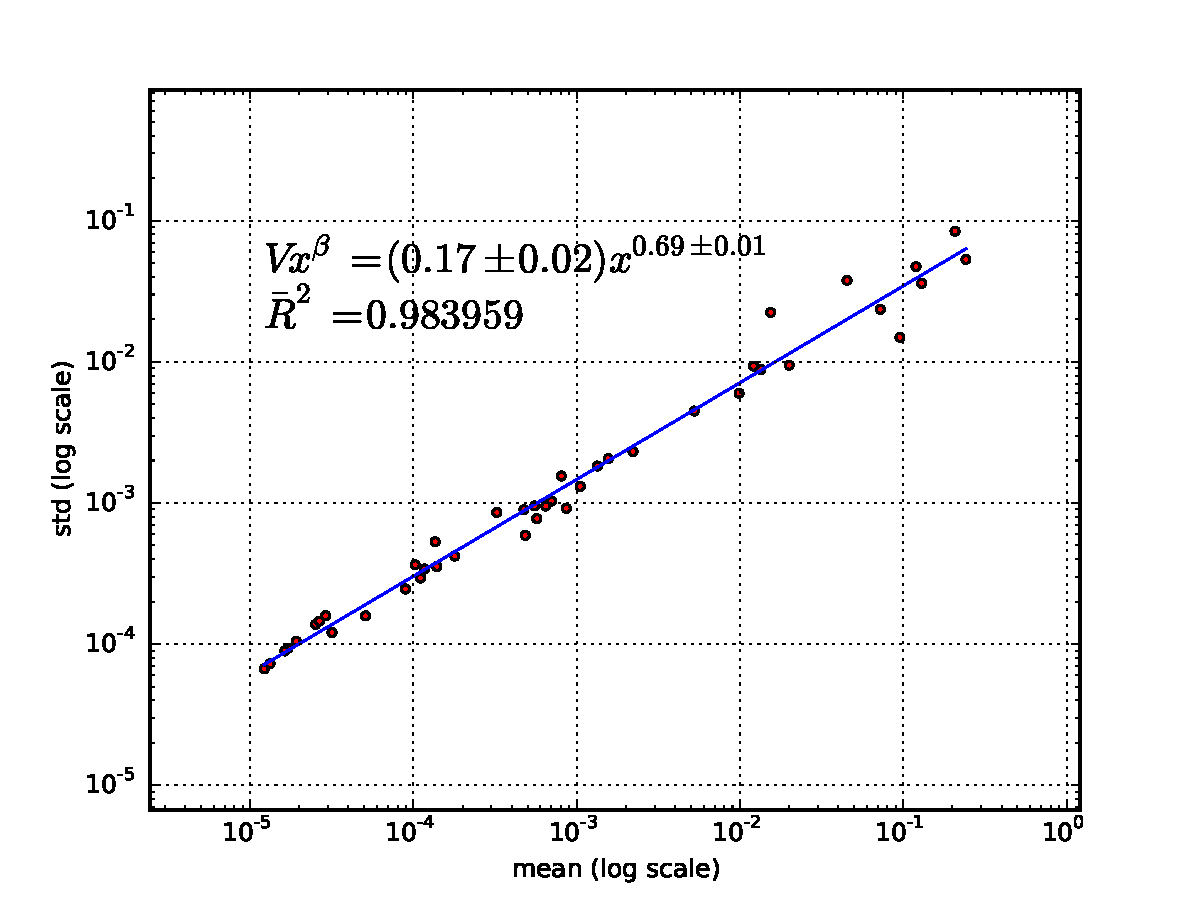
\includegraphics[width=0.8\textwidth]{results/fits/IBS_h_A_amplicons_family_stdVSmean_LLR_LOG.pdf}
	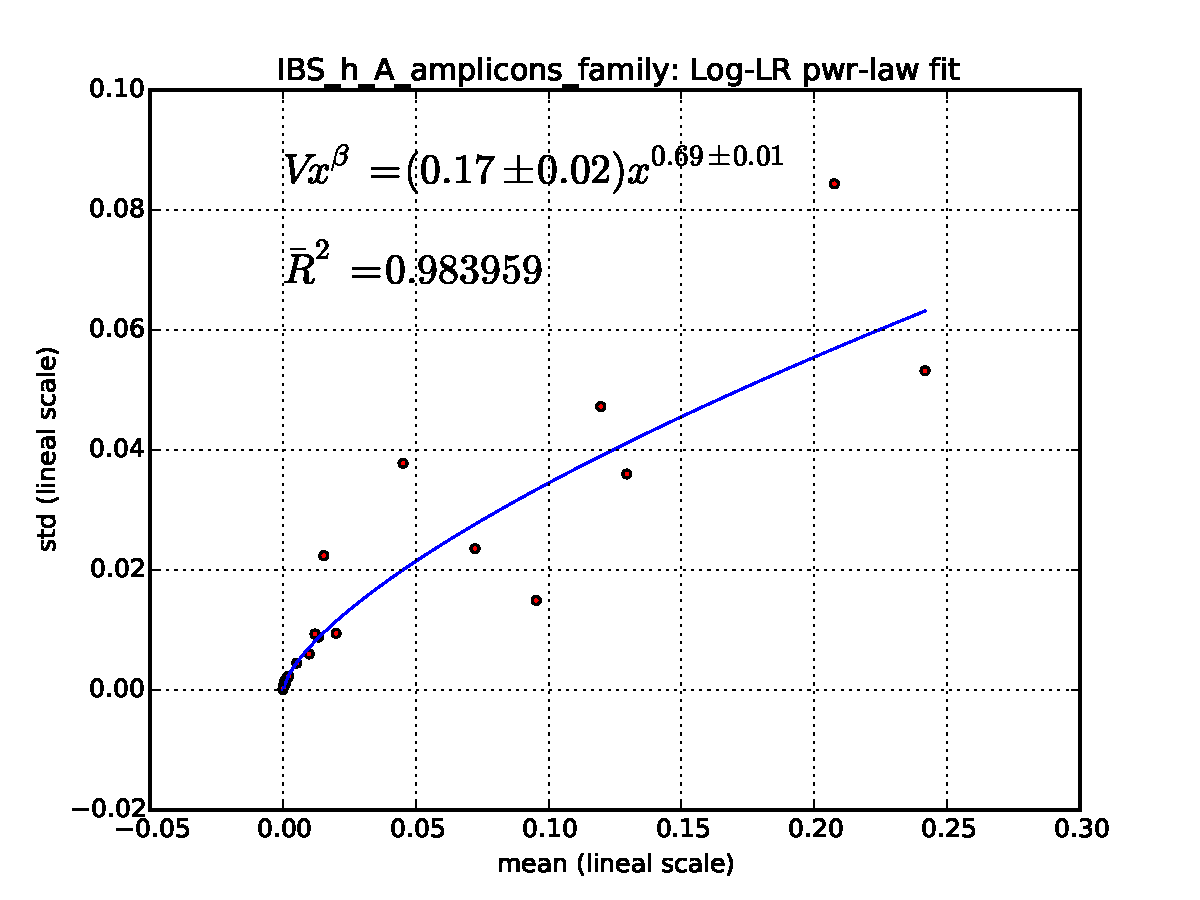
\includegraphics[width=0.8\textwidth]{results/fits/IBS_h_A_amplicons_family_stdVSmean_LLR_LIN.pdf}
	\caption{Example of unweighted fit, shown both in logarithmic and lineal scale plots}
	\label{fig:unwFit}
\end{figure}

\begin{figure}
	\centering
	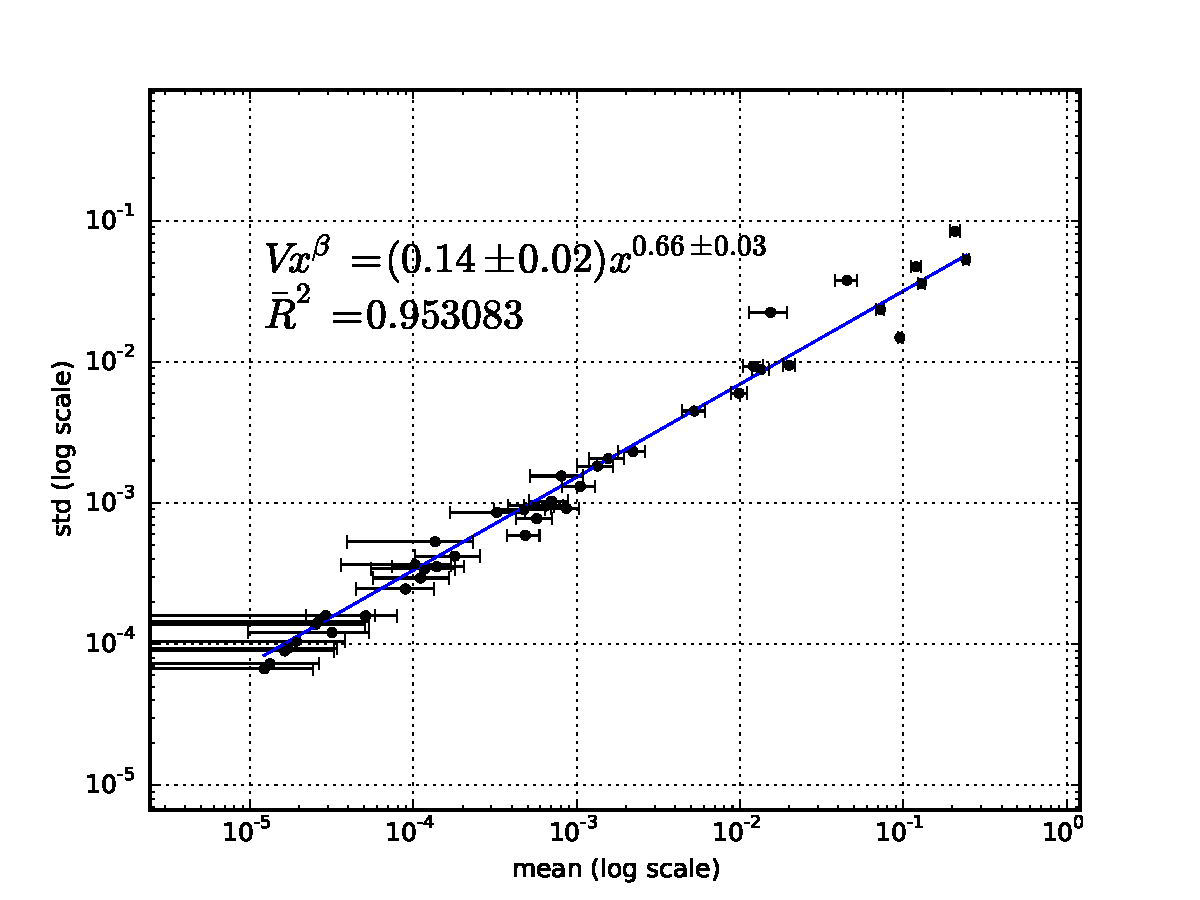
\includegraphics[width=0.8\textwidth]{results/fits/IBS_h_A_amplicons_family_stdVSmean_xWboot_LOG.pdf}
	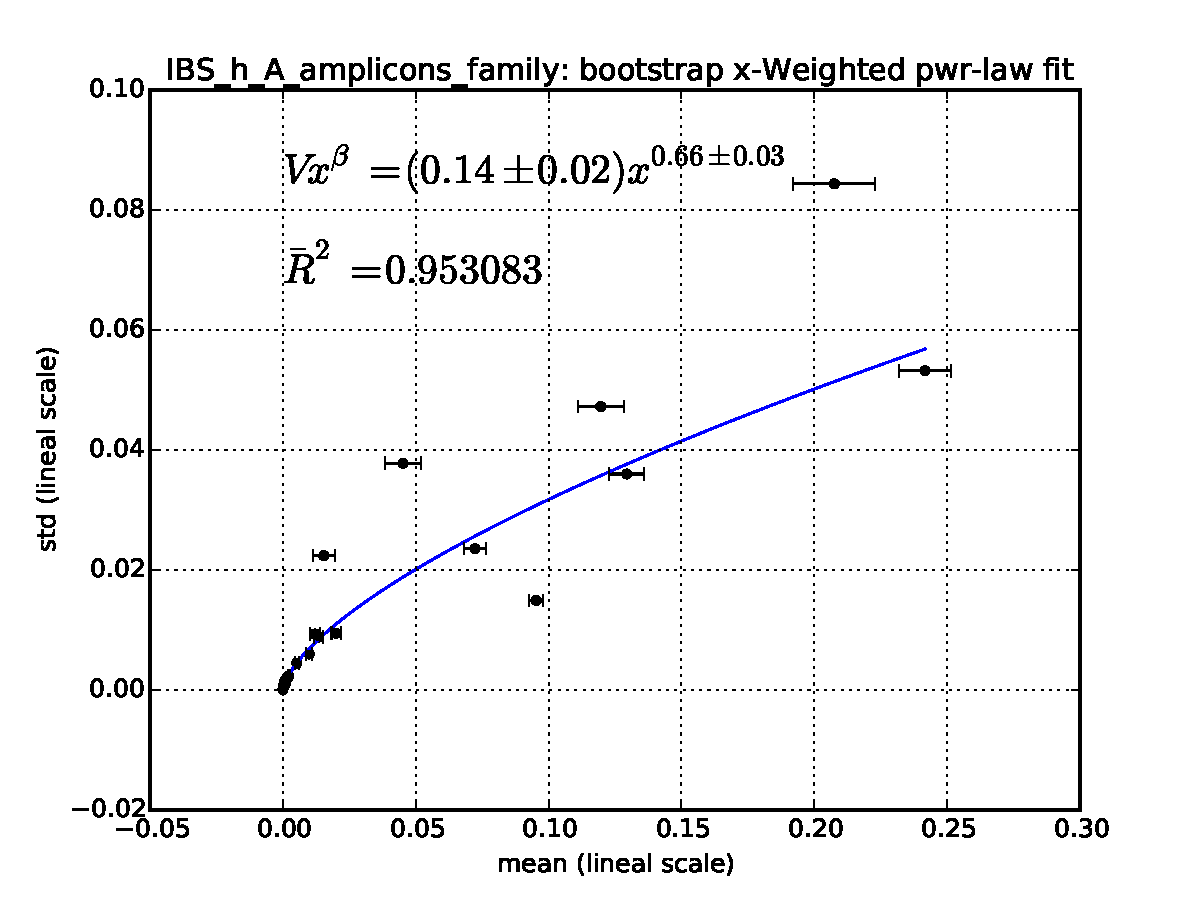
\includegraphics[width=0.8\textwidth]{results/fits/IBS_h_A_amplicons_family_stdVSmean_xWboot_LIN.pdf}
	\caption{The X-weighted fit log and lineal plots corresponding to the fit of Figure \ref{fig:unwFit}}
	\label{fig:X-wFit}
\end{figure}

\begin{figure}
	\centering
	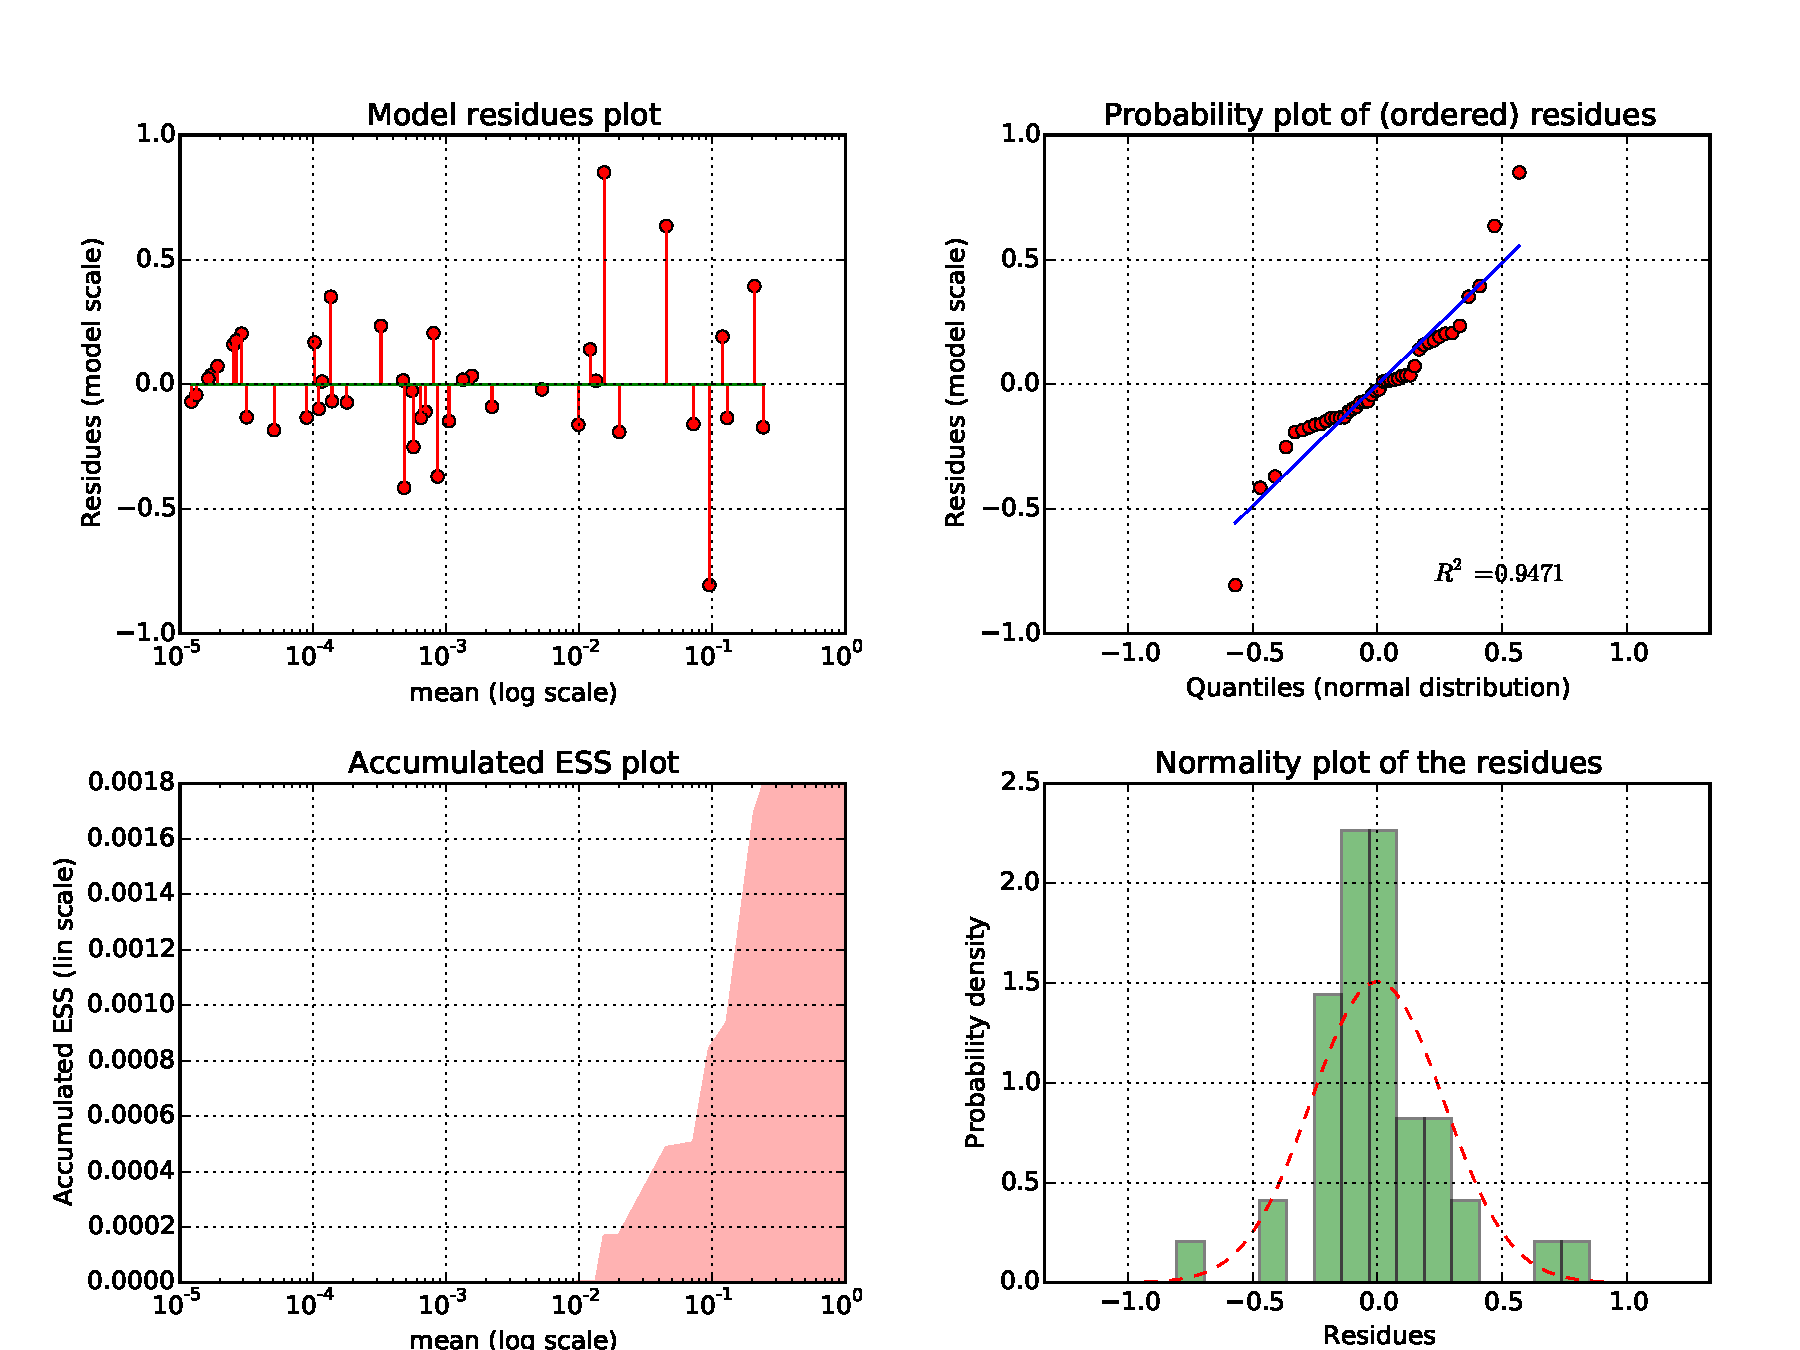
\includegraphics[width=\textwidth]{results/fits/IBS_h_A_amplicons_family_stdVSmean_LLR_RES.pdf}
	\caption{Residues analysis plot corresponding to the fit of Figure \ref{fig:unwFit}. The top-left subplot is a simple residues plot. The top-right subplot is a Normal quantiles plot with linear fitting (value of coefficient of determination is provided). The bottom-left subplot shows an accumulated ESS (Explained Sum of Squares) plot. Finally, the bottom-right subplot is a residues Normal histogram plot. This set of subplots allows to check for normality and homoscedasticity of the residues.}
	\label{fig:unwRes}
\end{figure}

\subsection{Histogram Plots} 
The subdirectory \texttt{hist} under the results directory contains the histogram plots. \CC\ generates three different histogram plots:
\begin{description}
	\item[$-$Absolute frequencies plot]: This plot is useful to visually assess the validity of the time points in terms of the accumulated absolute frequency of the elements (taxa), since absolute frequencies far (much higher or much lower) from those typically observed could mean a sampling problem. As an example, Figure \ref{fig:histAFP} shows this histogram for the pre-treatment data (first 7 times) of patient ``D'' in the antibiotics study\cite{antibiotic}. 
	\item[$-$2D deviation plot]: The 2D semi-logarithmic histogram representing deviations from the mean versus the mean itself, is a useful tool in the analysis of the stability of ranking processes in complex systems\cite{ranking}. Figure \ref{fig:hist2D} shows this plot for the data used in the fit shown in Figure \ref{fig:unwFit}.
	\item[$-$Zero relative frequency plot]: We could define the ZRF (Zero Relative Frequency, thereby ranging from 0 to 1) of an element (taxon) as the portion of times where it is zero, i.e., it is not found. Attending to all the elements (taxa), we can plot the ZRF histogram, which then lies on the horizontal axis of the plot. The vertical axis shows the number of elements (taxa), so the height of a bar represents the number of elements that have determinate ZRF. In this respect, the bar over $0.0$ counts the number of elements (taxa) that are present at every time point of the data set (aka ``core''), while the bar over $1.0$ would count the number of elements (taxa) that are never found (this bar never appears because all these ``null'' elements are automatically filtered by the code). Figure \ref{fig:histZRF} shows an example of this plot. There, we can see that $12$ taxa are present at all the time points of the time series while $9$ taxa basically appear only once. So, this plot is clearly useful to notice how the ``core'' is distributed.
\end{description}

\begin{figure}
	\centering
	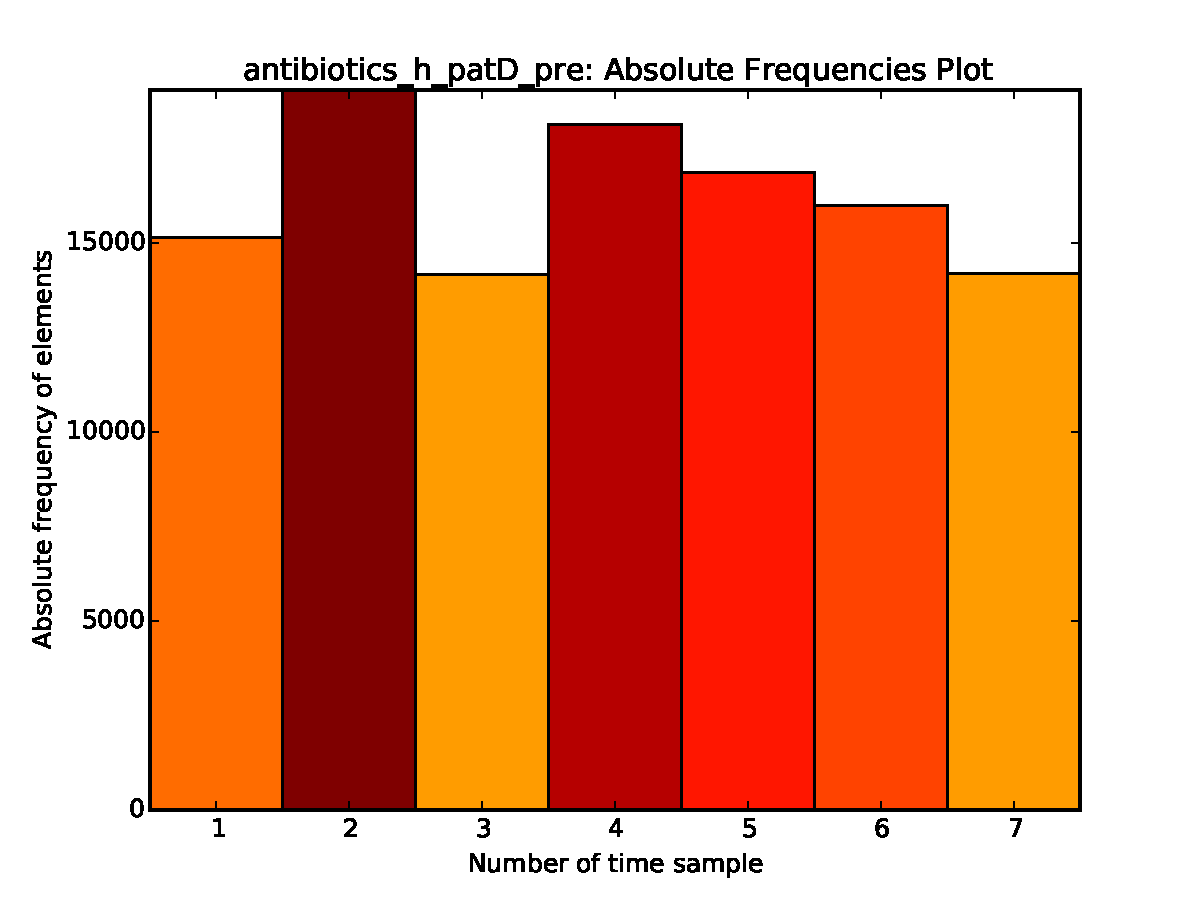
\includegraphics[width=0.8\textwidth]{results/hist/antibiotics_h_patD_pre_AbsFreqPlot}
	\caption{Histogram with the absolute frequencies of the pre-treatment data (7 first times) of patient ``D'' in the antibiotics study\cite{antibiotic}}
	\label{fig:histAFP}
\end{figure}

\begin{figure}
	\centering
	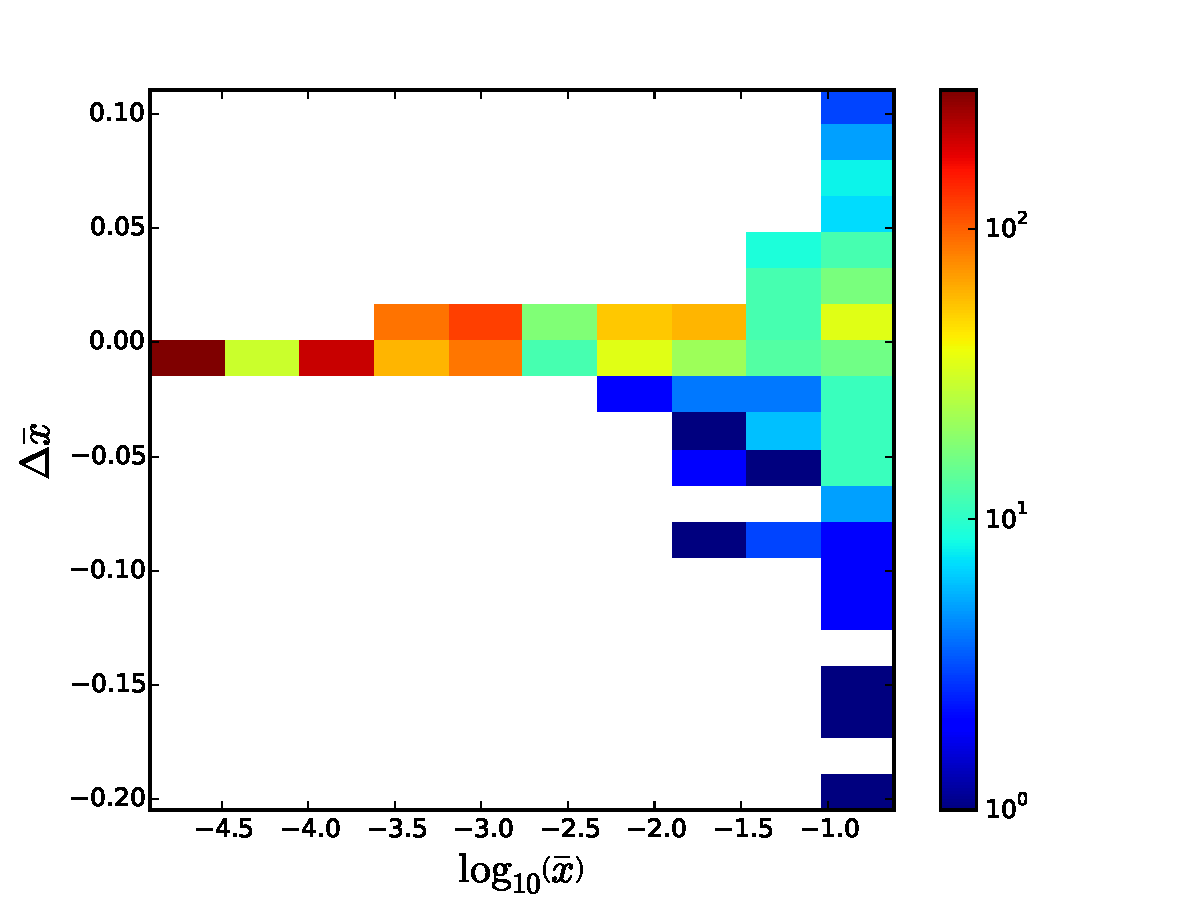
\includegraphics[width=0.8\textwidth]{results/hist/IBS_h_A_amplicons_family_hist2D.pdf}
	\caption{2D histogram deviation plot of the data used in the fit shown in Figure \ref{fig:unwFit}}
	\label{fig:hist2D}
\end{figure}

\begin{figure}
	\centering
	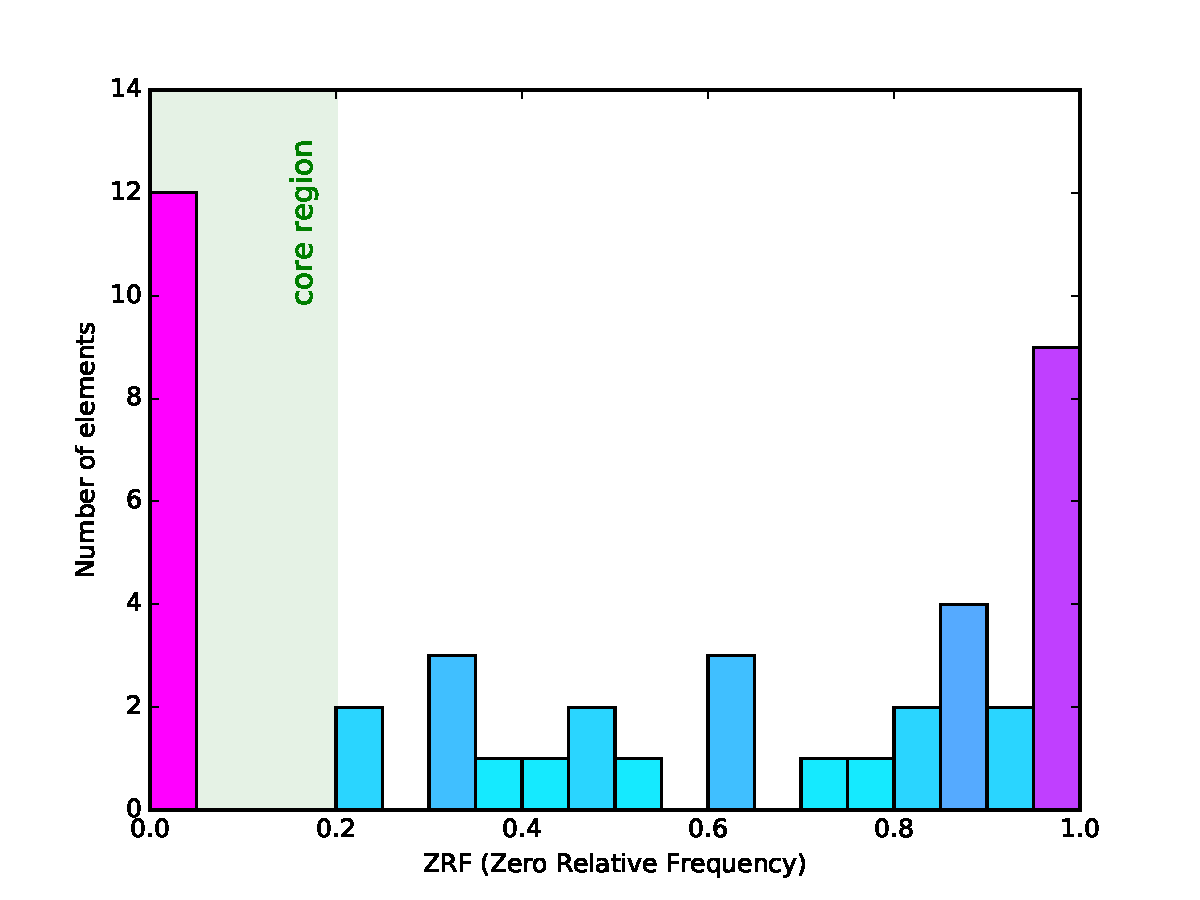
\includegraphics[width=0.8\textwidth]{results/hist/IBS_h_A_amplicons_family_ZRFhist.pdf}
	\caption{Histogram with the relative frequency of zero for the elements (taxa) in the data used in the fit shown in Figure \ref{fig:unwFit}}
	\label{fig:histZRF}
\end{figure}

\subsection{Correlation and Rank Plots} 
The subdirectory \texttt{corrank} under the results directory contains the correlation matrix and rank\&stability plots, as well as Excel files with the resulting matrices. \CC\ generates three different plots falling under this category:
\begin{description}
	\item[$-$Elements correlation matrix]: This plot shows a correlation matrix among the elements (taxa), calculated with the time as independent variable. For these calculations, the data set is not normalized to avoid entering an additional constraint. As an example, Figure \ref{fig:corrElm} shows this matrix for the ``core'' elements (taxa) present in the pre-treatment data (first seven times) of patient ``D'' in the antibiotics study\cite{antibiotic}. 
	\item[$-$Times correlation matrix]: This plot presents a correlation matrix among the time points of the data set, calculated with the elements (taxa) as independent variable. Again, the data set is not normalized. Figure \ref{fig:corrTim} shows this matrix for the ``core'' elements (taxa) present in pre-treatment data (first seven times) of patient ``D'' in the antibiotics study\cite{antibiotic}. 
	\item[$-$Rank dynamics and stability plot]: This plot shows the variation in the rank with time for the most dominant elements (taxa) and their calculated RSI, as discussed in Section \ref{sec:RSI}. Figure \ref{fig:corrank} shows this plot for the elements (taxa) in the data used in the fit shown in Figure \ref{fig:unwFit}.
\end{description}

\begin{figure}
	\centering
	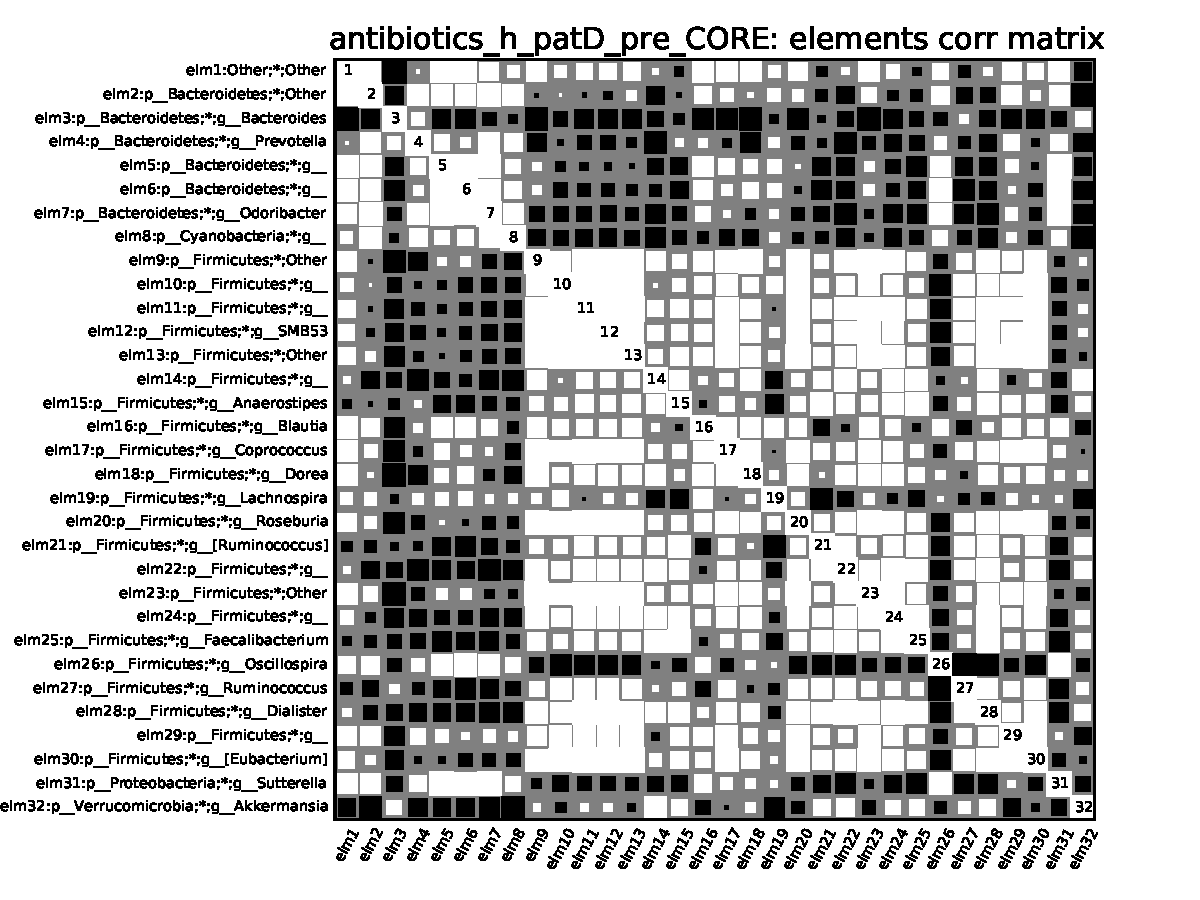
\includegraphics[width=0.9\textwidth]{results/corrank/antibiotics_h_patD_pre_CORE_ElementsCorr}
	\caption{Element correlation plot of the pre-treatment data (first seven times) of patient ``D'' in the antibiotics study\cite{antibiotic} for ``core'' taxa}
	\label{fig:corrElm}
\end{figure}

\begin{figure}
	\centering
	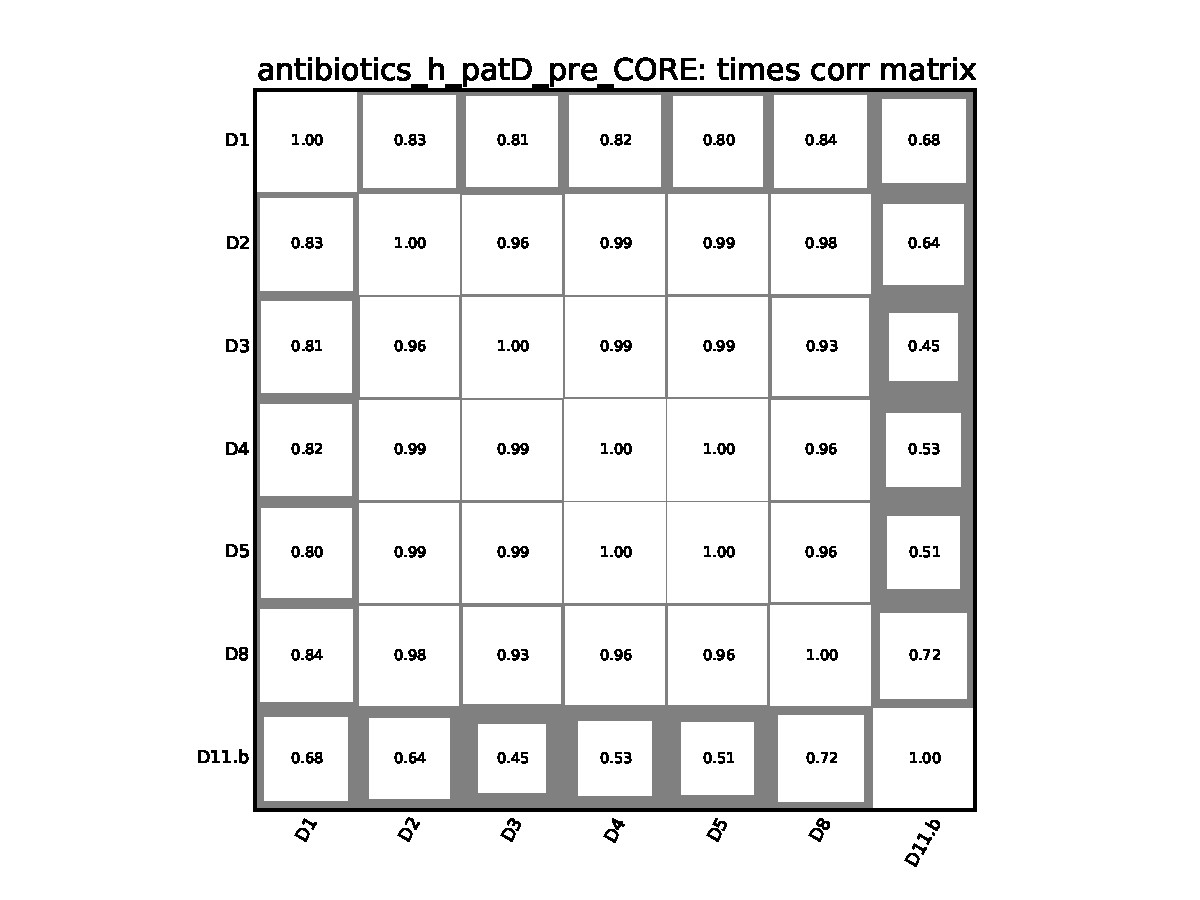
\includegraphics[width=0.9\textwidth]{results/corrank/antibiotics_h_patD_pre_CORE_TimesCorr}
	\caption{Times correlation plot of the pre-treatment data (first seven times) of patient ``D'' in the antibiotics study\cite{antibiotic} for ``core'' taxa}
	\label{fig:corrTim}
\end{figure}

\begin{figure}
	\centering
	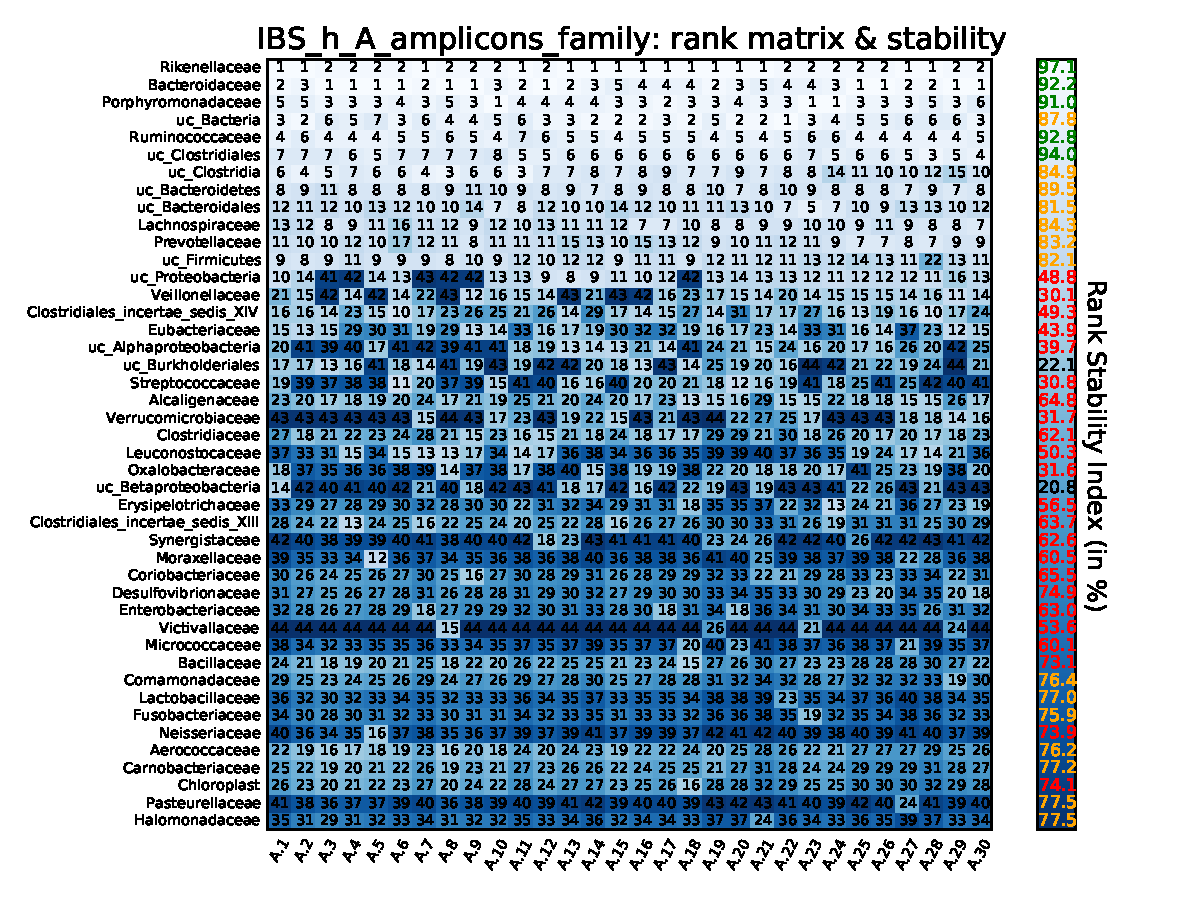
\includegraphics[width=\textwidth]{results/corrank/IBS_h_A_amplicons_family_Rank}
	\caption{Matrix showing the rank variation throughout time for the most dominant elements (taxa) and their calculated RSI (as discussed in Section \ref{sec:RSI}) in the data used in the fit shown in Figure \ref{fig:unwFit}}
	\label{fig:corrank}
\end{figure}

\subsection{Other Plots} 
The subdirectory \texttt{other} under the results directory contains other plots, like the elements (taxa) kurtosis and skewness against the mean. These plots are generated when the flag \texttt{-m}/\texttt{--more} is given to the \CC.py front-end script.

\subsection{\CC\ advanced options}
The advanced option flags are summarized here:
\begin{description}
	\item[$-$ZRF filter]: This is activated with \texttt{-c}/\texttt{--core} and allows global and detached results for ``core'', ``tailless'' and ``tail'', which allows comparative analysis depending on the presence/absence rate of the taxa throughout time, which is calculated in practice using the Zero Relative Frequency (ZRF) defined above. The criteria is as follows: 
	\begin{itemize}
		\item In any case, if $\operatorname{ZRF} < 0.2$ taxa are classified as ``core''. In other words, the taxa considered ``core'' are those appearing at over $80\%$ of the time points under analysis.
		\item Depending on the number of times:
		\begin{itemize}
			\item If there are only 3 time points, taxa with $0.2 \le\operatorname{ZRF} < 0.4$ are classified as ``tailless'' and, therefore, taxa with $\operatorname{ZRF} \ge 0.4$ are classified as ``tail''.
			\item If there are 4 time points, taxa with $0.2 \le\operatorname{ZRF} < 0.5$ are classified as ``tailless'' and, therefore, taxa with $\operatorname{ZRF} \ge 0.5$ are classified as ``tail''.
			\item If there are 5 or more time points, taxa with $0.2 \le\operatorname{ZRF} < 0.6$ are classified as ``tailless'' and, therefore, taxa with $\operatorname{ZRF} \ge 0.6$ are classified as ``tail''.			      
		\end{itemize}
    \end{itemize}
	\item[$-$Relative frequency filters]: The minimum frequency filter is activated with \texttt{-z}/\texttt{--fmin} and the maximum one with \texttt{-x}/\texttt{--fmax}, with values between $0$ and $1$. If both filters are activated simultaneously, the minimum frequency cannot be equal or higher than the maximum one. If no filter is activated, by default, \CC\ is filtering all the taxa that never appear throughout time, in the event there are such taxa among the input data. On the one hand, if a minimum frequency value is provided, all the taxa whose relative accumulated frequencies (the normalized sum of the values through time) are under such a value, are eliminated. But in addition, once the set of data is normalized (to work with relative frequencies), if there are data at any time points that are under the minimum frequency given value, they are automatically floored to zero (we call this \emph{item@time filtering}), and the set of data is renormalized. On the other hand, if a maximum frequency value is provided, all the taxa whose relative accumulated frequencies are over such value, are deleted. 
\end{description}

\section{\CC\ input}
The input data are provided by two simultaneously available ways:
\begin{enumerate}
	\item Text files (\texttt{txt} extension), to be processed in parallel\footnote{Currently, parallelization in \CC\ is only available under GNU/Linux}, with a shared-memory model.
	\item Excel files (\texttt{xls[x]} extension), whose sheets are related datasets to be processed in parallel\footnotemark[\value{footnote}]. Optionally, all the sheets of an Excel file are standardized using part of such Excel datasets, following the procedure described in the Supplementary Section \ref{sec:stan}, in which event, additional output is provided by \CC.
\end{enumerate}
Typically, the data sets are tables with the taxa lying in different rows and the time points ordered in different columns. So, the first column is considered the taxon labels, whereas the first row contains the time labels. It is worth mentioning that any Excel sheet or text file beginning with the underscore character is ignored by \CC, as they are supposed to hold metadata.

\section{Standardization} \label{sec:stan}
In order to show all the studies properly under common axes, we decided to standardize the Taylor parameters using the group of healthy individuals for each study. With this approach, all the studies can be visualized in a shared plot with units of Taylor-parameters standard-deviation on their axes.

For a Taylor parameter, e.g. $V$, the estimate of the mean ($\widehat{V}$) for the healthy subpopulation, composed of $h$ individuals, is:
$$\widehat{V} = \frac{1}{W_1}\sum_{i=1}^h V_i \omega_i=\sum_{i=1}^h V_i \omega_i$$
as $W_1=\sum_i^h \omega_i=1$, since $\omega_i$ are normalized weights calculated as:
$$\omega_i = \frac{\frac{1}{\sigma^2_{V_i}}}{\sum_i^h\frac{1}{\sigma^2_{V_i}}}$$
being $\sigma_{V_i}$ the estimation of the uncertainty in $V_i$ obtained together with $V_i$ from the X-weighted power-law fit described in Section \ref{sec:X-w}, for healthy individuals.

Likewise, the estimation of the standard deviation for the healthy population ($\widehat{\sigma}_V$) is:
$$\widehat{\sigma}_V = \sqrt{\frac{1}{W_1-\frac{W_2}{W_1}}\sum_{i=1}^h\left[\omega_i\left(V_i-\hat{V}\right)^2\right]}$$
being $W_2=\sum_i^h \omega_i^2$, which finally yields to:
$$\widehat{\sigma}_V = \sqrt{\frac{1}{1-\sum_i^h \omega_i^2}\sum_{i=1}^h\left[\omega_i\left(V_i-\hat{V}\right)^2\right]}$$

\section{\CC\ interface with LMAT} \label{sec:lmat}
With the aim of adapting LMAT (Livermore Metagenomics Analysis Toolkit) software\cite{LMAT} for its easy use in time series data, like the ones we have analyzed in this paper\cite{kwashiorkor}, we developed Python front and back-end scripts. They are supplied in the directory \texttt{tools} of the \CC\ package.

\subsection{LMAT front-ends} They are: \texttt{pyLMAT\_rl.py}, the launcher for LMAT \texttt{run\_rl.sh}, that is, the first step in the LMAT pipeline or \emph{read labeling}; \texttt{pyLMAT\_cs.py}, the launcher for LMAT \texttt{run\_cs.sh}, the \emph{content summarization} step in the LMAT pipeline; and, \texttt{pyLMAT\_gl.py}, the launcher for LMAT \texttt{run\_gl.sh}, the \emph{gene labeling/identification} step in the LMAT pipeline. Basically, all three scripts permit to manage the execution of parallelized LMAT against several fasta files coming from diferent time points in time series studies.

\subsection{LMAT back-ends} Currently, they are: \texttt{pyLMAT\_rescore.py} and the pipeline composed by \texttt{rawlmat2lmat.py} and \texttt{lmat2cmplx.py}. The first one allows not only to quick recalculate the LMAT results for different cutoff levels, but also to pull out reads with specific NCBI taxId (\emph{human} reads by default). For example, issuing "\texttt{pyLMAT\_rescore.py -p path/to/results -f file.fna -m -1 0 1 -t=32}" will regenerate the LMAT results for cutoffs $-1$, $0$ and $1$, and will pull human reads for each cutoff level, parallelizing in $32$ threads. On the other hand, the mentioned pipeline enables to post-process the several \emph{fastsummary} output files from LMAT first and second steps launched by the LMAT front-ends described above. The pipeline transforms the results so that they achieve a format and content ready for \CC\ computations. Such data arrangements are done independently for two different taxonomic levels: genus and specie.

\newpage
\begin{thebibliography}{1}
	\bibitem{ranking} Blumm, N. \textit{et al.} Dynamics of ranking processes in complex systems. {\it Phys. Rev. Lett.} {\bf 109,} 128701 (2012).
	\bibitem{FD} Weber, J. \textit{et al.} Fluctuation dissipation theorem. {\it Phys. Rev.} {\bf 101}, 1620-6 (1956).
	\bibitem{kwashiorkor} Smith M.I.  \textit{et al.} Gut microbiomes of Malawian twin pairs discordant for kwashiorkor. {\it Science} {\bf 339,} 548-54 (2013).
	\bibitem{FASTX} Gordon, A., Hannon, G.J. FASTX-Toolkit. FASTQ/A shortreads pre-processing tools (2010). http://hannonlab.cshl.edu/fastx\_toolkit/ (accessed 23 Feb 2015).
	\bibitem{QIIME} Caporaso, J.G. \textit{et al.} QIIME allows analysis of high-throughput community sequencing data. {\it Nature Methods} {\bf 7,} 335-6 (2010).
	\bibitem{SILVA} Quast C.  \textit{et al.} The SILVA ribosomal RNA gene database project: improved data processing and web-based tools (2013)
	\bibitem{LMAT} Ames, S.K.  \textit{et al.} Scalable metagenomic taxonomy classification usng a reference genome database. {\it Bioinformatics} {\bf 29,} 2253-2260 (2013).
	\bibitem{antibiotic} Dethlefsen L., Relman D. A. Incomplete recovery and individualized responses of the human distal gut microbiota to repeated antibiotic perturbation. {\it Proc. Nat. Acad. Sci. USA} {\bf 108,} 4554-61 (2011).
	\bibitem{diet} David, L.A. \textit{et al.} Diet rapidly and reproducibly alters the human gut microbiome. {\it Nature} {\bf 505,} 559-63 (2014).
	\bibitem{IBS} Durban, A. \textit{et al.} Structural alterations of faecal and mucosa-associated bacterial communities in irritable bowel syndrome. {\it FEMS Microbiol. Ecol.} {\bf 86}, 581-9 (2013).
	\bibitem{LEA} Faith, J.J.  \textit{et al.} The long-term stability of the human gut microbiota. {\it Science} {\bf 341,} 1237439 (2013).
	\bibitem{moving} Caporaso, J.G.  \textit{et al.} Moving pictures of the human microbiome. {\it Genome Biol.} {\bf 12,} R50 (2011).
 	\bibitem{ecology} Xiao Xiao, Ethan P. White, Mevin B. Hooten, and Susan L. Durham. On the use of log-transformation vs. nonlinear regression for analyzing biological power laws. {\it Ecology} {\bf 92}, 10, 1887-1894 (2011).
 	\bibitem{genR2} Magee L., $R^2$ measures based on wald and likelihood ratio joint significance tests. {\it The American Statistician} {\bf 44}, 3, 250-253 (1990).
	\bibitem{disR2} Nagelkerke N.J.D., A note on a general definition of the coefficient of determination. {\it Biometrika} {\bf 78}, 3, 691-692 (1991).
	\bibitem{boot} Wu, C.F.J. Jackknife, bootstrap and other resampling methods in regression analysis. (with discussions) \textit{The Annals of Statistics} {\bf 14}: 1261?1350 (1986)
\end{thebibliography}


\end{document}




































